


\section{Measurement}

    All plots and the raw data of all experiments are accessible on Sciebo in Ref. \cite{sciebo_data}. (Last access September 2026) \\

    For a measurement on a given cylinder $D$ for an array of droplet volumes $V$, the cylinder is cleaned using the wipes and fixed on the platform using rubber bands. Measurements of $W$ in the front position (\cref{fig:photo_measure}, left) are performed separately from measurements of $L$ in the side position (\cref{fig:photo_measure}, right) on different droplets. Therefore, no pair of $L$ and $W$ belong to the  same droplet. To make up for this lack of correspondence, each measurement is performed $4$ to $5$ times and averaged. \\

    To place the droplets on the cylinder, one of two procedures is used:
    \begin{enumerate}
        \item The full volume of the droplet is placed on the cylinder at once, measured, cleaned off, and replaced by the next droplet volume of interest. This method is precise, but slow as the focus has to be readjusted each time. It is used for small cylinders $D < \SI{4}{mm}$.
        \item A \SI{2}{mm} droplet is placed, measured, and incremented to fit the next droplet volume of interest. The incrementation and measurement are repeated until the droplet becomes unstable and slides off the cylinder. This method is fast, but accumulates error due to the repeated manipulation of the droplet. It is used for large cylinders $D \geq \SI{4}{mm}$.
    \end{enumerate}
    It is assumed that the cylinder substrates do not \enquote{memorize} the exposure to previously applied droplets such that no additional waiting time is needed between measurements. \\

    \Cref{fig:example_2mm_2ul} shows an exemplary measurement on the \SI{2}{\milli\meter} cylinder, using the procedure (1) for a \SI{2}{\micro\liter} droplet. On PMMA, the experiment was repeated fordroplet volumes \SI{2.2}{\micro\liter}, \SI{2.4}{\micro\liter}, \SI{2.6}{\micro\liter}, \SI{2.9}{\micro\liter}, and \SI{3.2}{\micro\liter}. Due to the limitations of the pipette, drop volumes below \SI{2}{\micro\liter} were inaccessible.
    \begin{figure}[H]
        \centering
        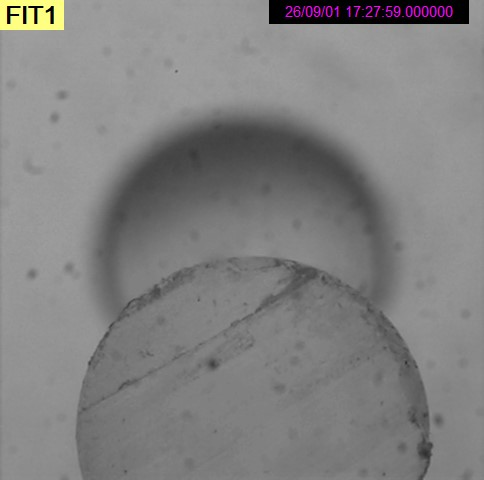
\includegraphics[width=0.32\linewidth]{../Figs/Meas_PMMA_02mm_front-1.jpg}
        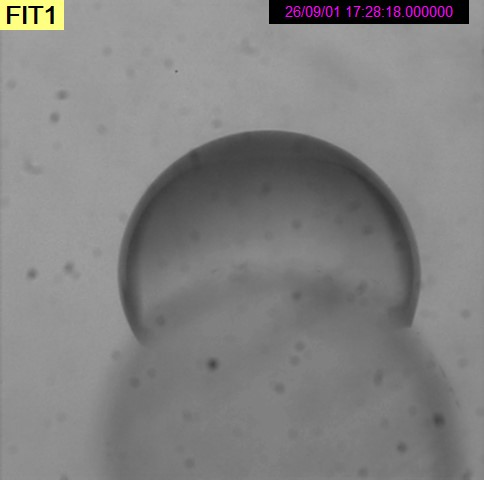
\includegraphics[width=0.32\linewidth]{../Figs/Meas_PMMA_02mm_front-2.jpg}
        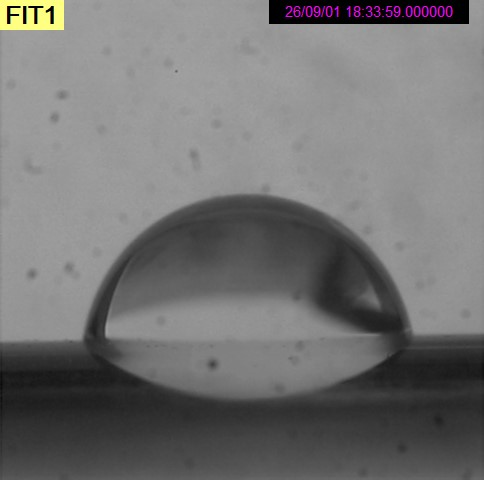
\includegraphics[width=0.32\linewidth]{../Figs/Meas_PMMA_02mm_side-1.jpg}
        \caption{Measurement of a \SI{2}{\micro\liter} droplet on the \SI{2}{\milli\meter} cylinder from the front (left, middle) and side perspective (right). }
        \label{fig:example_2mm_2ul}
    \end{figure}
    On the \SI{4}{\milli\meter} PMMA/PET cylinder (\cref{fig:example_4mm_6ul}), procedure (2) was used, incrementing a \SI{2}{\micro\liter} droplet to \SI{4}{\micro\liter}, \SI{6}{\micro\liter}, \SI{8}{\micro\liter}, \SI{10}{\micro\liter}, and \SI{12}{\micro\liter}. The \SI{12}{\micro\liter} measurement, however, showed repeated instability and therefore cannot be analyzed. 
    \begin{figure}[H]
        \centering
        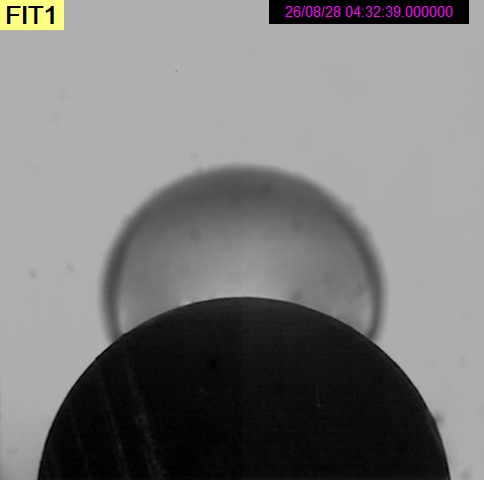
\includegraphics[width=0.49\linewidth]{../Figs/Meas_PMMA_04mm_front-1.jpg}
        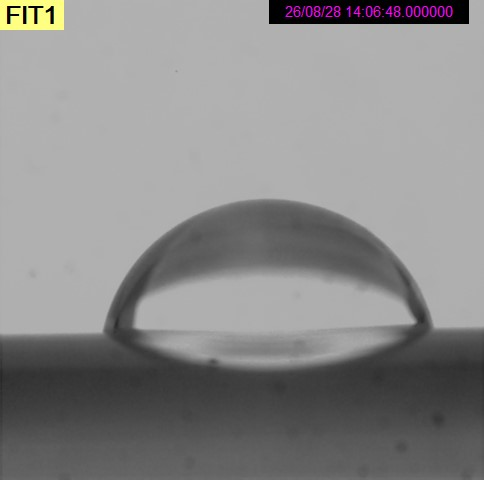
\includegraphics[width=0.49\linewidth]{../Figs/Meas_PMMA_04mm_side-1.jpg}
        \caption{Measurement of a \SI{6}{\micro\liter} droplet on the \SI{4}{\milli\meter} cylinder from the front (left) and side perspective (right). }
        \label{fig:example_4mm_6ul}
    \end{figure}
    Similarly, on the \SI{10}{\milli\meter} cylinder (\cref{fig:example_10mm_16ul}), procedure (2) was used, incrementing a \SI{2}{\micro\liter} droplet to \SI{4}{\micro\liter}, \SI{8}{\micro\liter}, \SI{12}{\micro\liter}, \SI{16}{\micro\liter}, \SI{20}{\micro\liter}, and \SI{30}{\micro\liter}. The \SI{30}{\micro\liter}, however, showed repeated instability and therefore cannot be analyzed. 
    \begin{figure}[H]
        \centering
        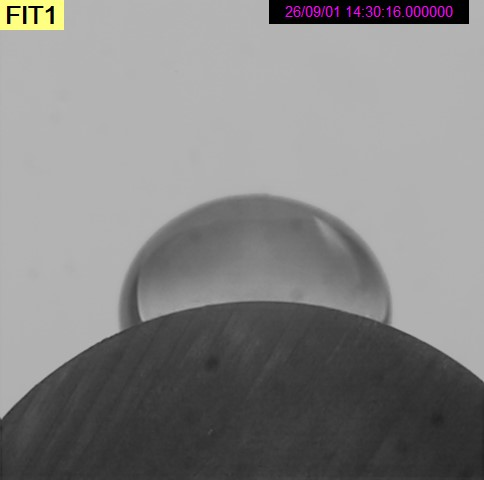
\includegraphics[width=0.49\linewidth]{../Figs/Meas_PMMA_10mm_front-1.jpg}
        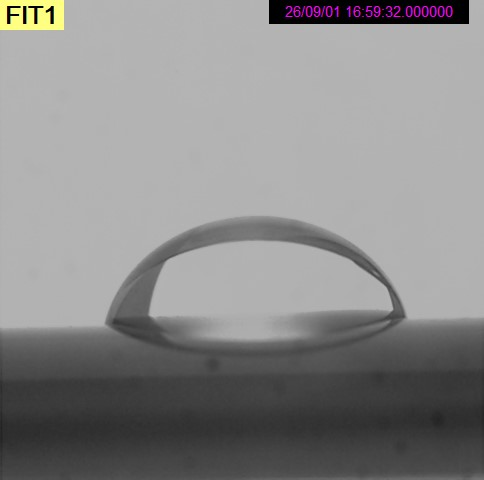
\includegraphics[width=0.49\linewidth]{../Figs/Meas_PMMA_10mm_side-1.jpg}
        \caption{Measurement of a \SI{16}{\micro\liter} droplet on the \SI{10}{\milli\meter} cylinder from the front (left) and side perspective (right). }
        \label{fig:example_10mm_16ul}
    \end{figure}
    Note that due to the short focus length of the camera, it was not always possible to focus the droplet's silhouette and the cylinder at the same time. In these cases, the focus on the cylinder is preferred as it showed to be more precise and reliable than focusing the droplets individually.

    \begin{figure}[H]
        \centering
        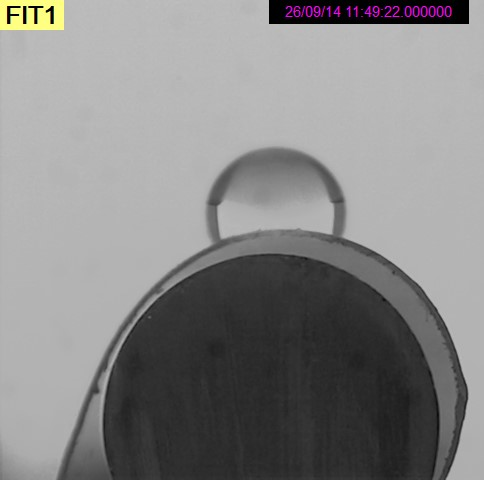
\includegraphics[width=0.49\linewidth]{../Figs/Meas_PET_04mm.jpg}
        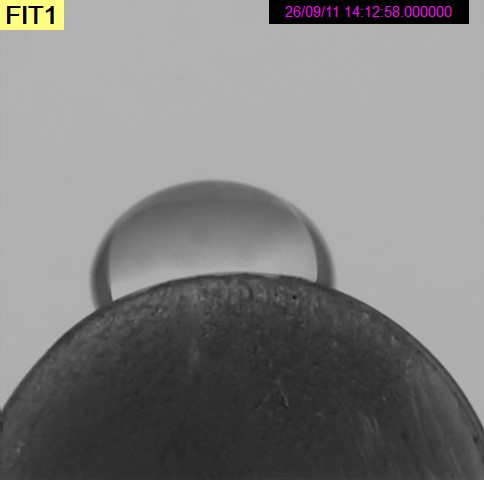
\includegraphics[width=0.49\linewidth]{../Figs/Meas_PET_10mm.jpg}
        \caption{Measurement on the \SI{4}{\milli\meter} (left) and \SI{10}{\milli\meter} PET cylinder (right). While the sample quality of the \SI{10}{\milli\meter} cylinder does not show immediate problems, the \SI{4}{\milli\meter} cylinder with PET foil shows visible deviations. The effective diameter of this cylinder is measured as \SI{4.08(20)}{\milli\meter}.}
        \label{fig:example_PET}
    \end{figure}

    We assume a relative uncertainty of \SI{5}{\percent} for all lengths measured in the images ($L$, $x$, gauge pipe) due to the limitations of the camera focus and image quality. Moreover, this uncertainty is meant to compensate for small deviations in droplet volume and induced vibrations during droplet placement. Generally speaking, there are countless possible sources of systematic error such as changes in room temperature and humidity, pollution of the sample and liquid, inaccurate camera placement, and evaporation. We nevertheless believe that the dominant source of uncertainty is caused by the droplet placement and sample impurity. 

\section{Results}
\subsection{Measurements on PMMA}

    \Cref{fig:PMMA_L} shows the contact lengths $L$ measured for different cylinder diameters $D$ or equivalently different curvatures $K = 1/D$. 
    \begin{figure}[H]
        \centering
        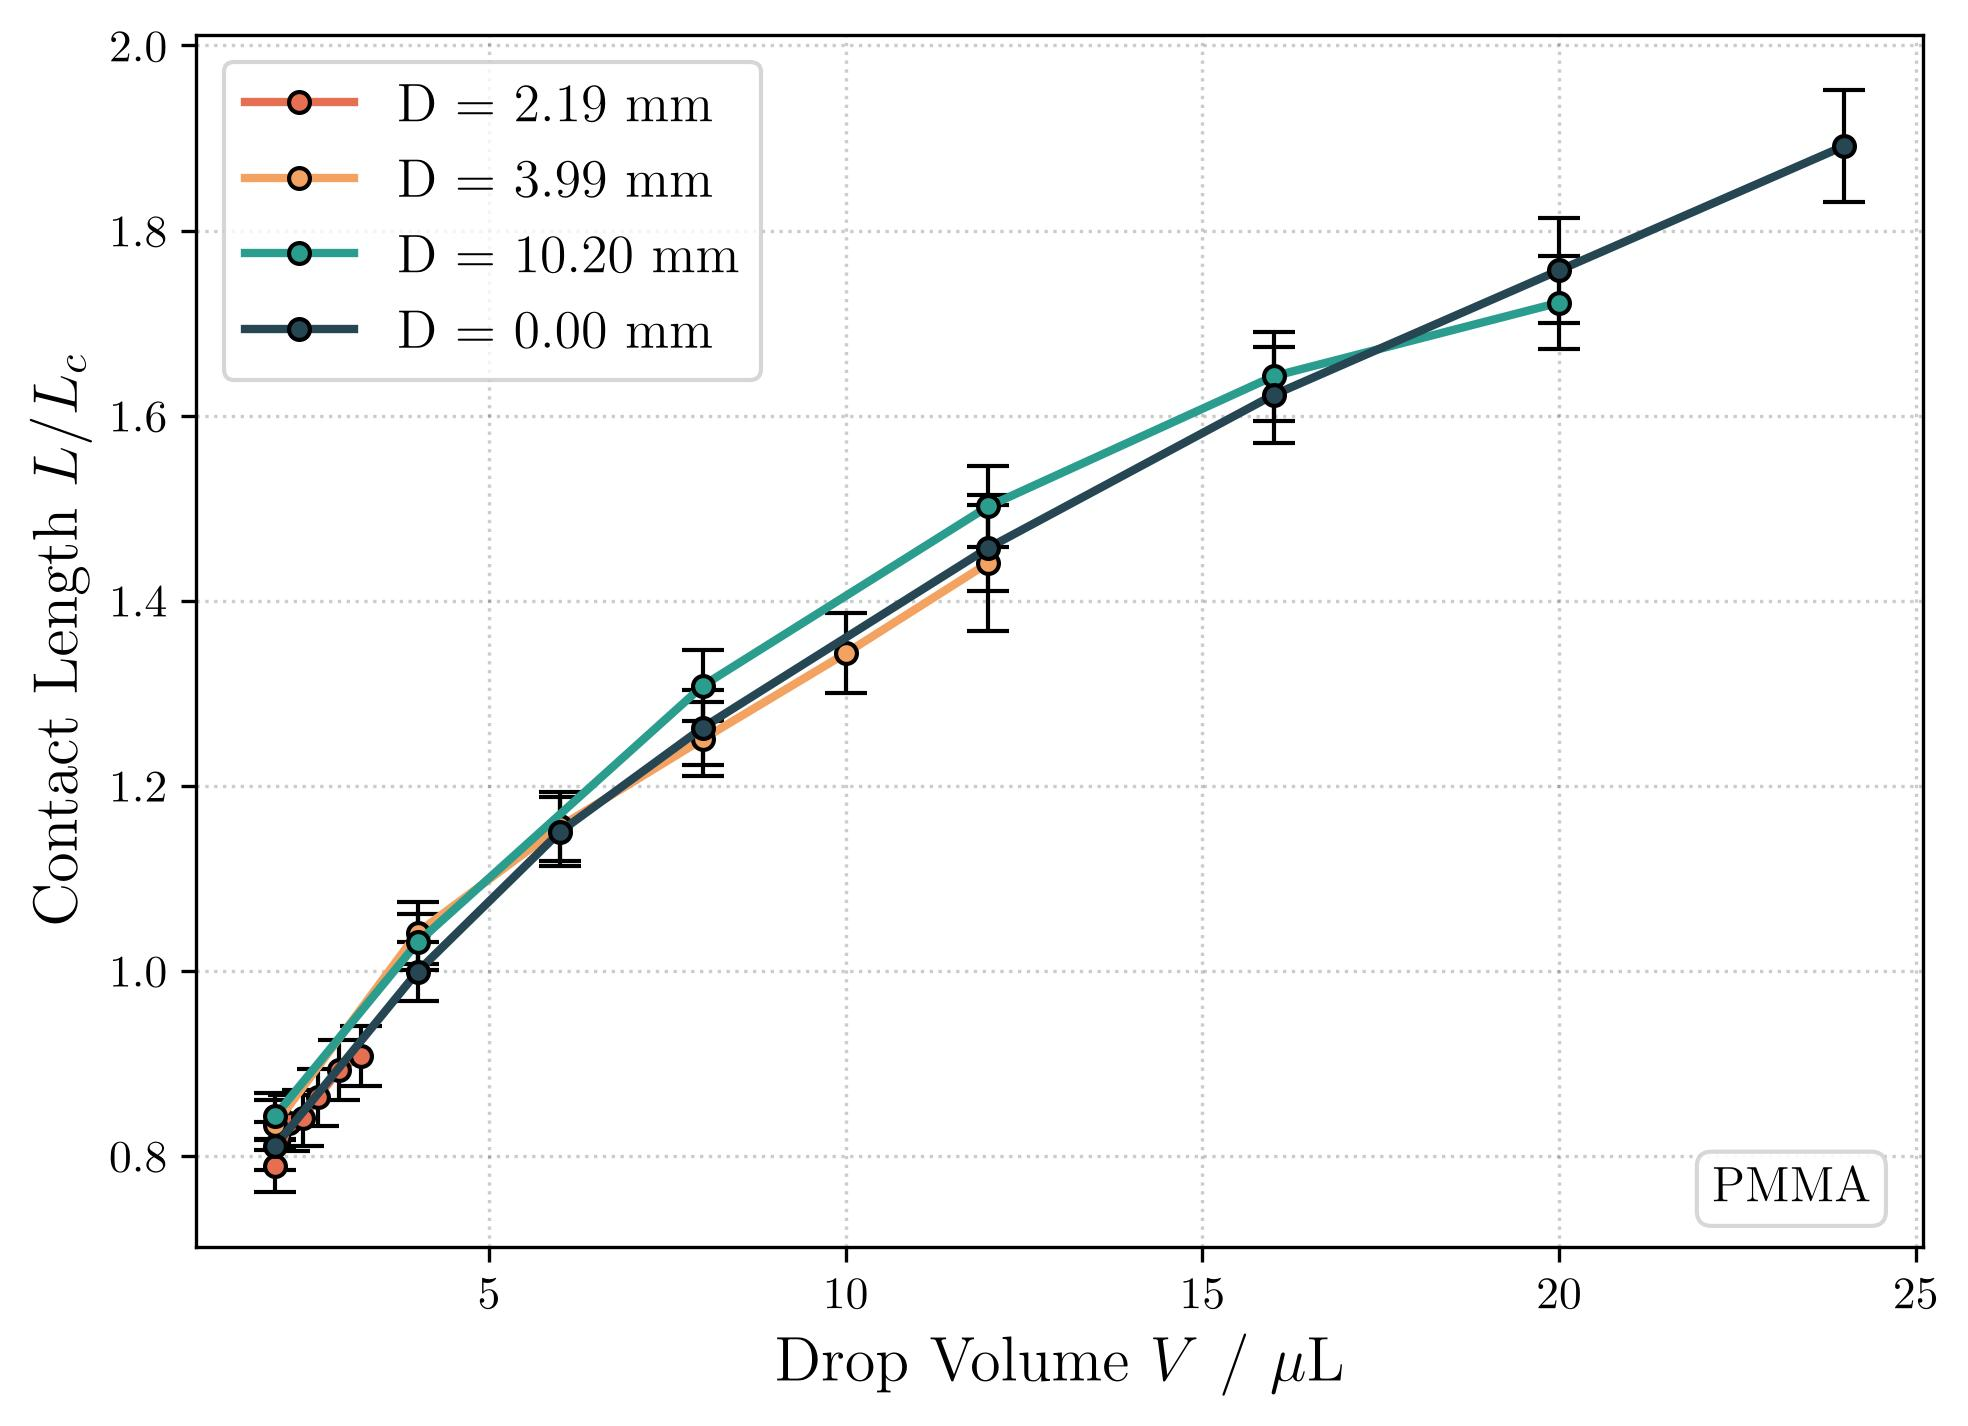
\includegraphics[width=\linewidth]{../Plots/w06_PMMA_L.jpg}
        \caption{Contact lengths $L$ on PMMA for different diameters $D$. Each data point is averaged over 4 - 7 measurement repetitions.}
        \label{fig:PMMA_L}
    \end{figure}
    It is clearly visible that all measurements follow a global trend which can be qualitatively described as a logarithmic curve. In this respect, the data points for each volume align by less than two standard deviations, indicating that there is a direct relationship between the two input parameters droplet volume $V$ and cylinder diameter $D$. Surprisingly, however, the measurement on the flat surface $(D = \SI{0.00}{\milli\meter})$ is not easily distinguishable from other measurements and instead shows intersection with other measurements. 
    \begin{figure}[H]
        \centering
        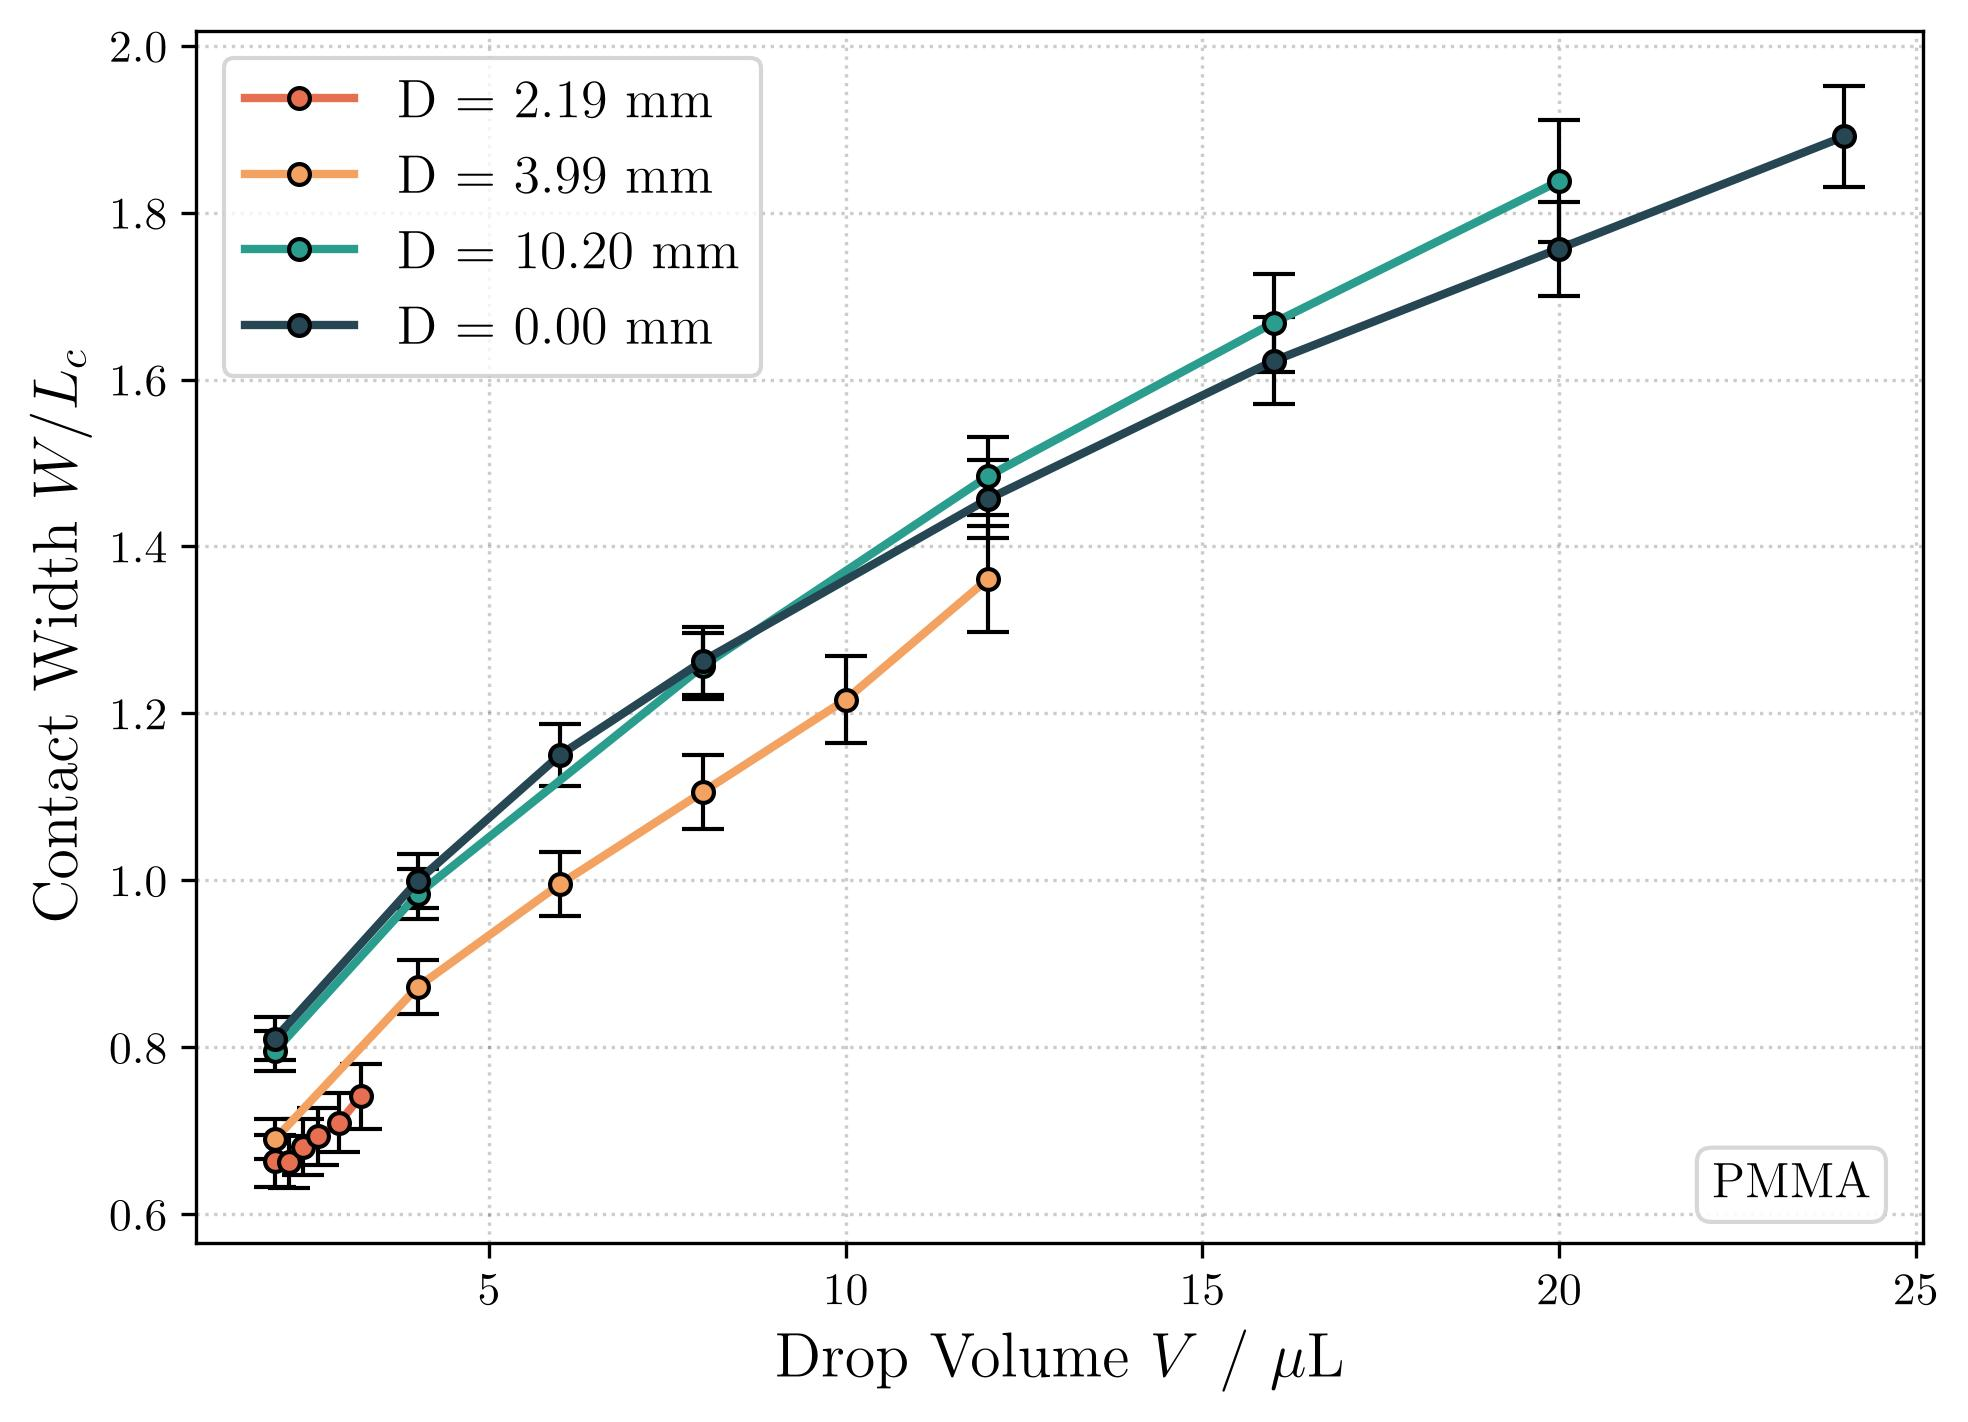
\includegraphics[width=\linewidth]{../Plots/w06_PMMA_W.jpg}
        \caption{Contact Widths $W$ on PMMA for different diameters $D$. Each data point is averaged over 4 - 7 measurement repititions.}
        \label{fig:PMMA_W}
    \end{figure}
    One possible reason for this might be the appearance of some tipping point where the balance between surface tension and gravity changes (for the cylinders but not for the flat surface).
    Another explanation suggests a systematic error from the measurement: even on the flat surface, it was observed how droplets formed asymmetrically due to placement-induced vibrations and pinning effects. It is therefore necessary to repeat the measurement using automatic droplet placement in order to eliminate the concern completely. \\ 

    The latter observations can also be made for the contact widths $W$ in \cref{fig:PMMA_W}. However, here, the contact widths on small cylinders deviate more from comparable measurements on large cylinders. This can be explained by the fact that $W$ is more prone to curvature-induced effects, such as the droplet sliding down on the sides. 
    \begin{figure}[H]
        \centering
        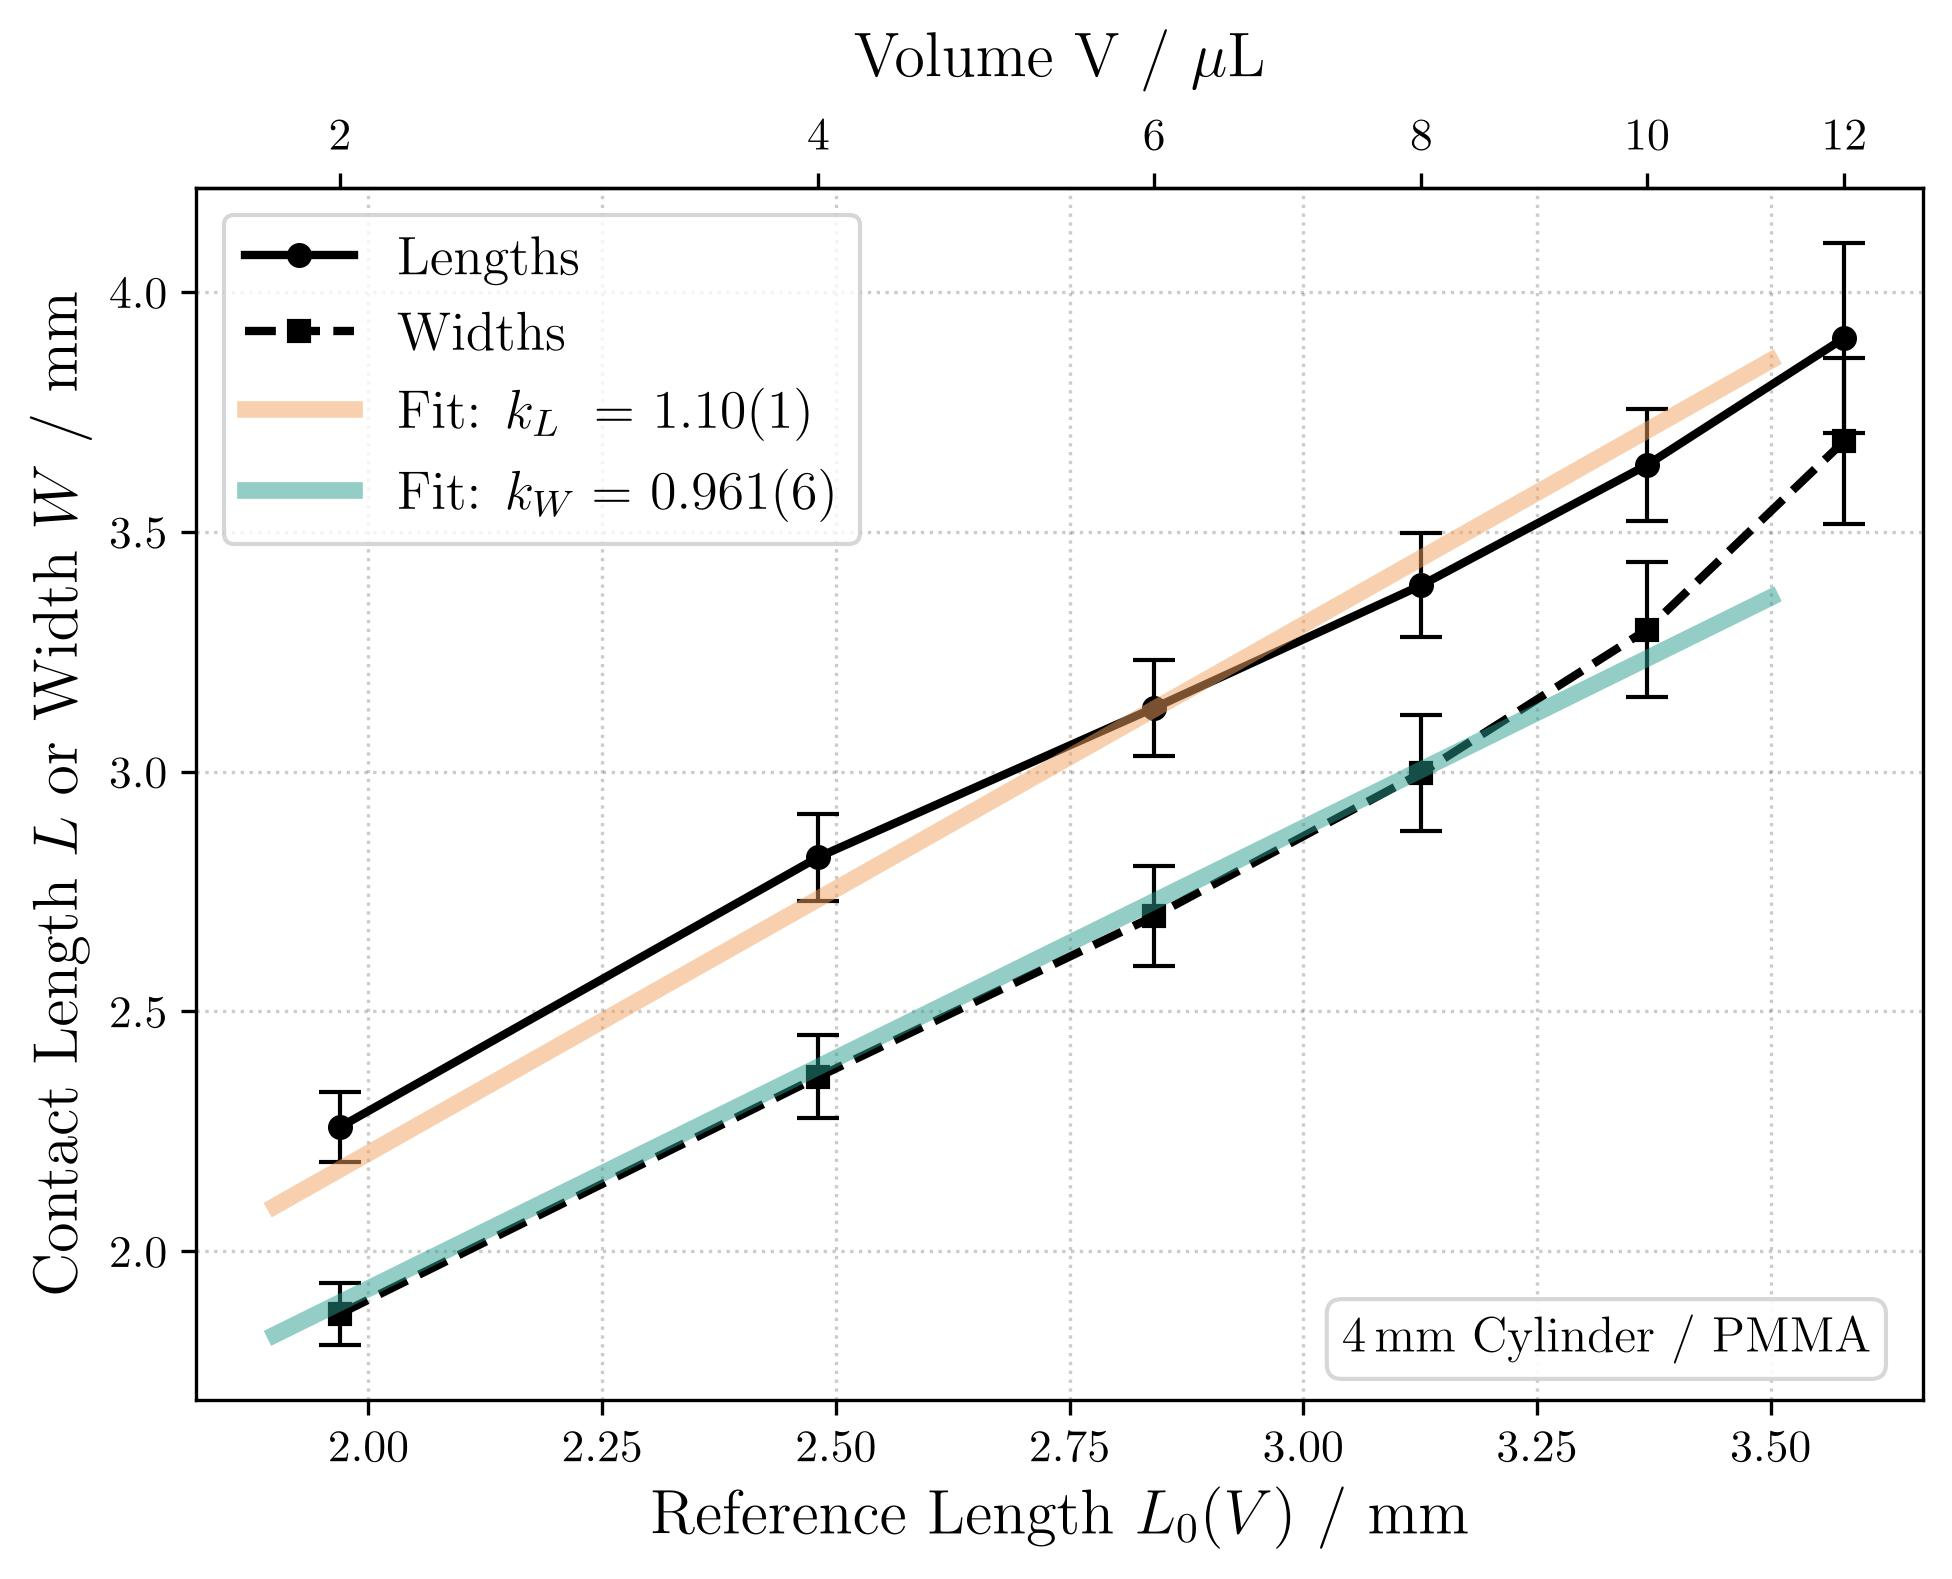
\includegraphics[width=\linewidth]{../Plots/w06_04mm_PMMA_L+W_fit.jpg}
        \caption{Contact lengths $L$ and widths $W$ on the \SI{4}{\milli\meter} PMMA cylinder, plotted against the reference length $L_0(V)$.}
        \label{fig:PMMA_04mm_fit}
    \end{figure}
    When it comes to the comparison of contact lengths and widths to the droplet volume, we want to use the quantitative measurement of the droplet shape compared to a half-sphere of the same volume, as discussed in \cref{sec:theory} and \cref{eq:L_and_W_against_L0}. \Cref{fig:PMMA_04mm_fit} shows as an example how the half-sphere model correctly describes the data with $k_L \sim k_W \sim 1$ as expected. The linear model starts deviating from the experiment in the regime where gravity dominates and the droplet starts sliding off to the side ($V = \SI{12}{\micro\liter}$ is excluded from the linear fit). \\
    
    To gauge the linear model and to show what the influence of curvature has to compare to, we apply the model to the contact length on a flat PMMA surface $(D \to \infty)$ as depicted in \cref{fig:PMMA_00mm_fit}.
    \begin{figure}[H]
        \centering
        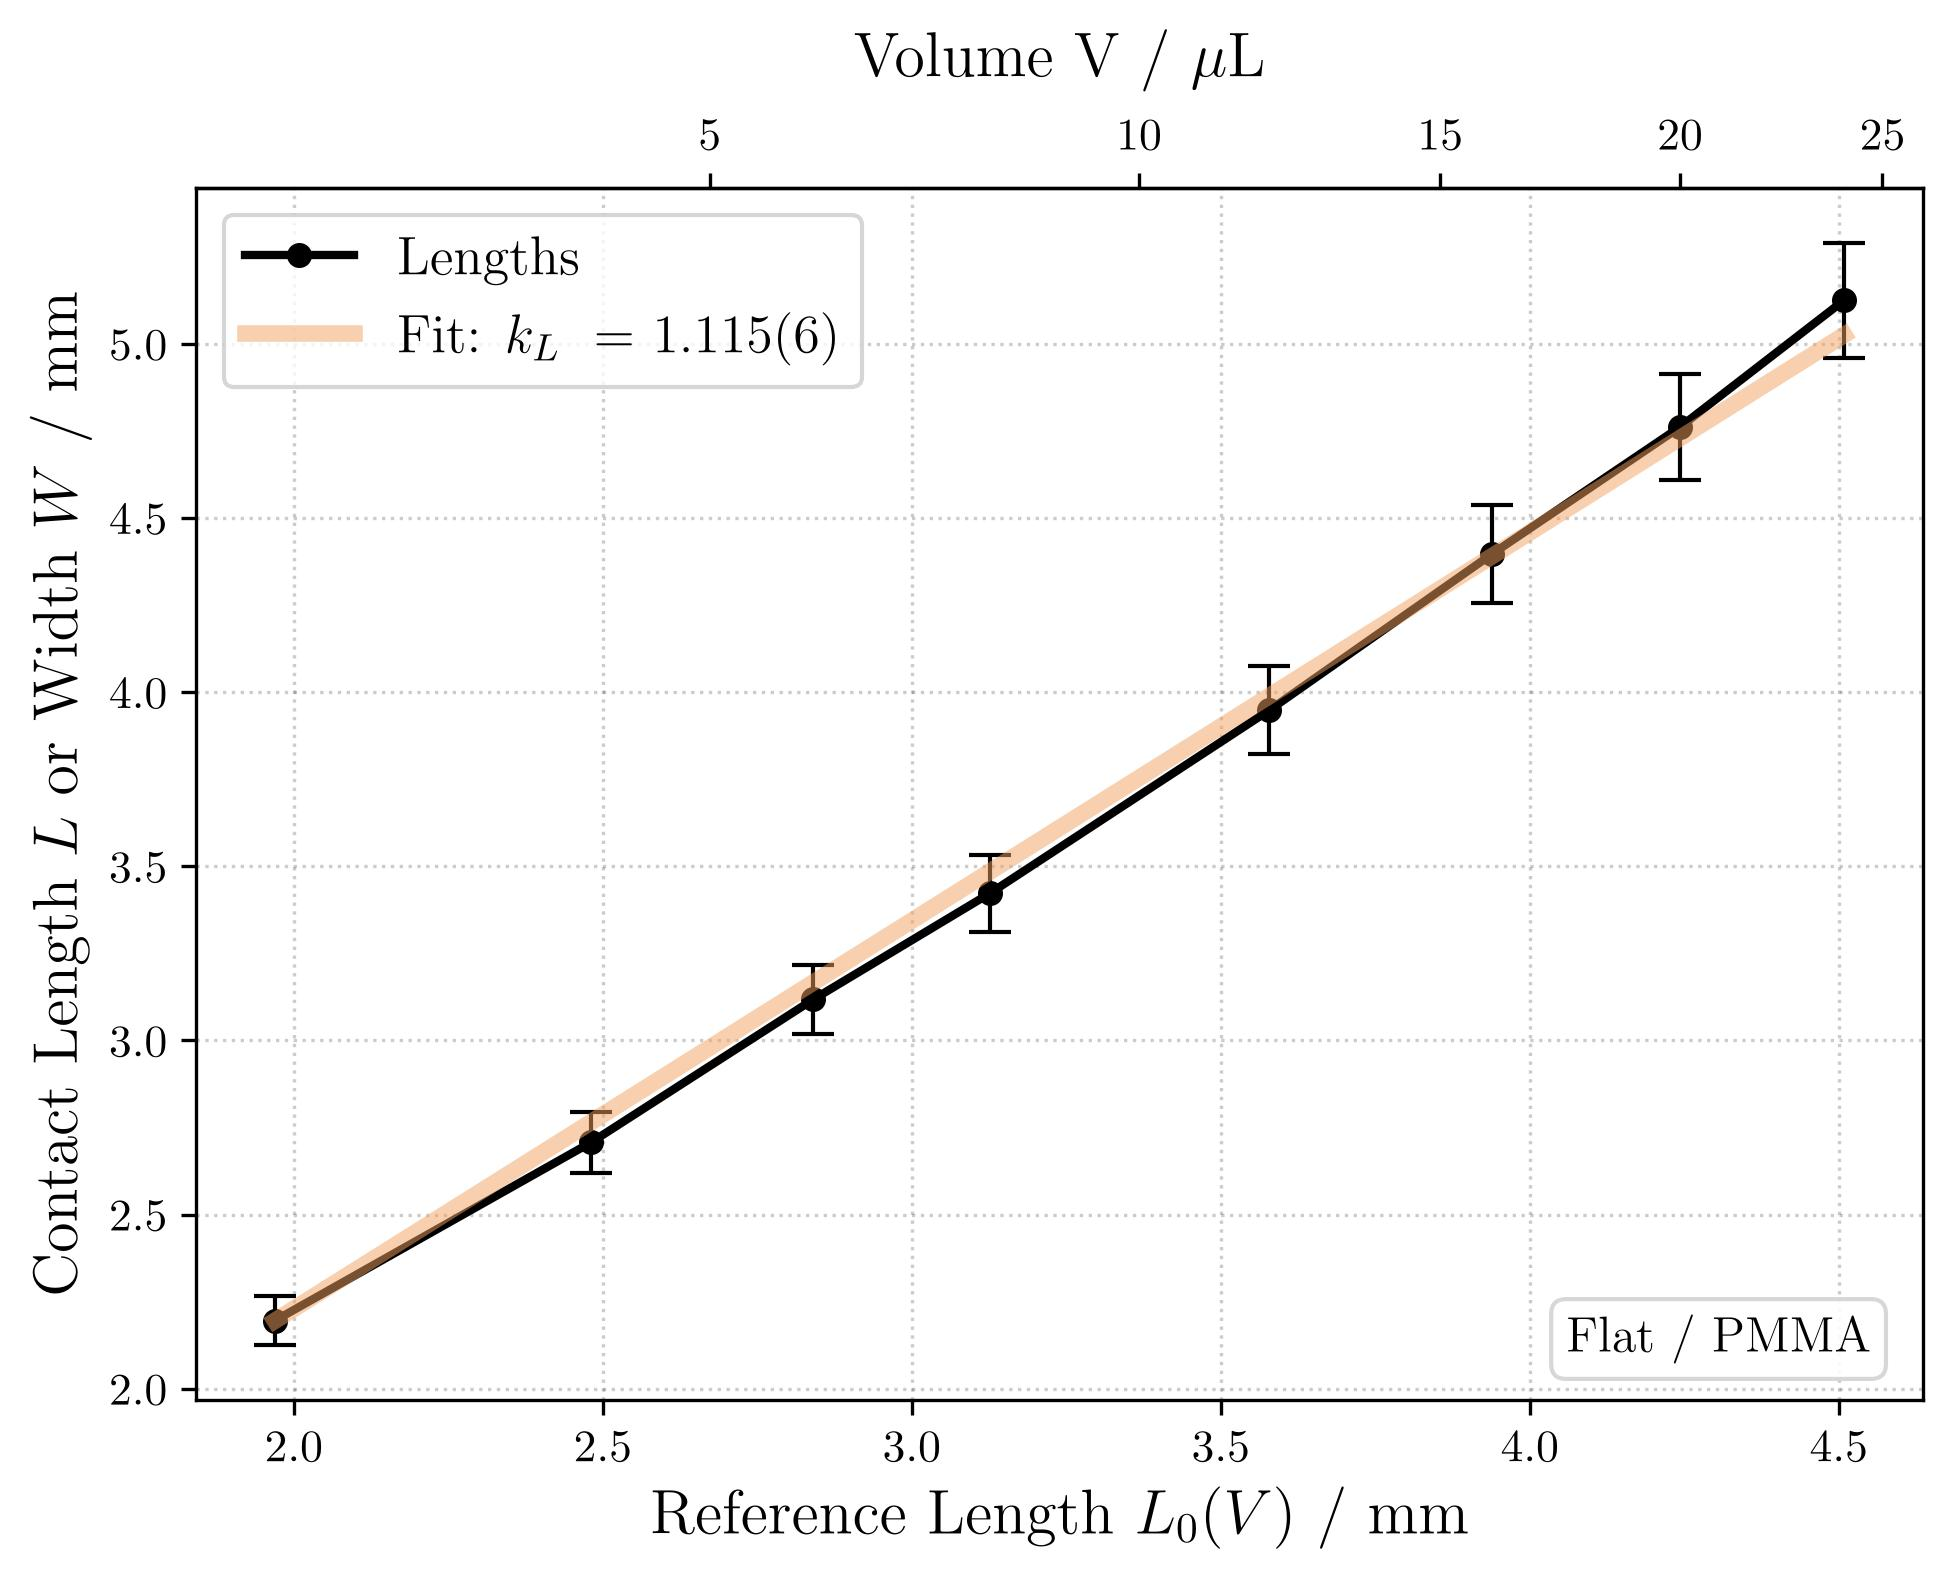
\includegraphics[width=\linewidth]{../Plots/w06_flat_PMMA_L_fit.jpg}
        \caption{Contact lengths $L$ on the flat PMMA cylinder, plotted against the reference length $L_0(V)$.}
        \label{fig:PMMA_00mm_fit}
    \end{figure}
    The high agreement of the linear trend with the data supports the claim that the half-sphere model is a functioning effective description of the droplet shape on a relatively hydrophobic surface. The slope of $k_L = \num{1.115(6)} > 1$ is a material-dependent parameter and the fact that it is greater than $1$ indicates a \enquote{flattened} shape with contact angles below \SI{90}{\degree}.    
    \begin{figure}[H]
        \centering
        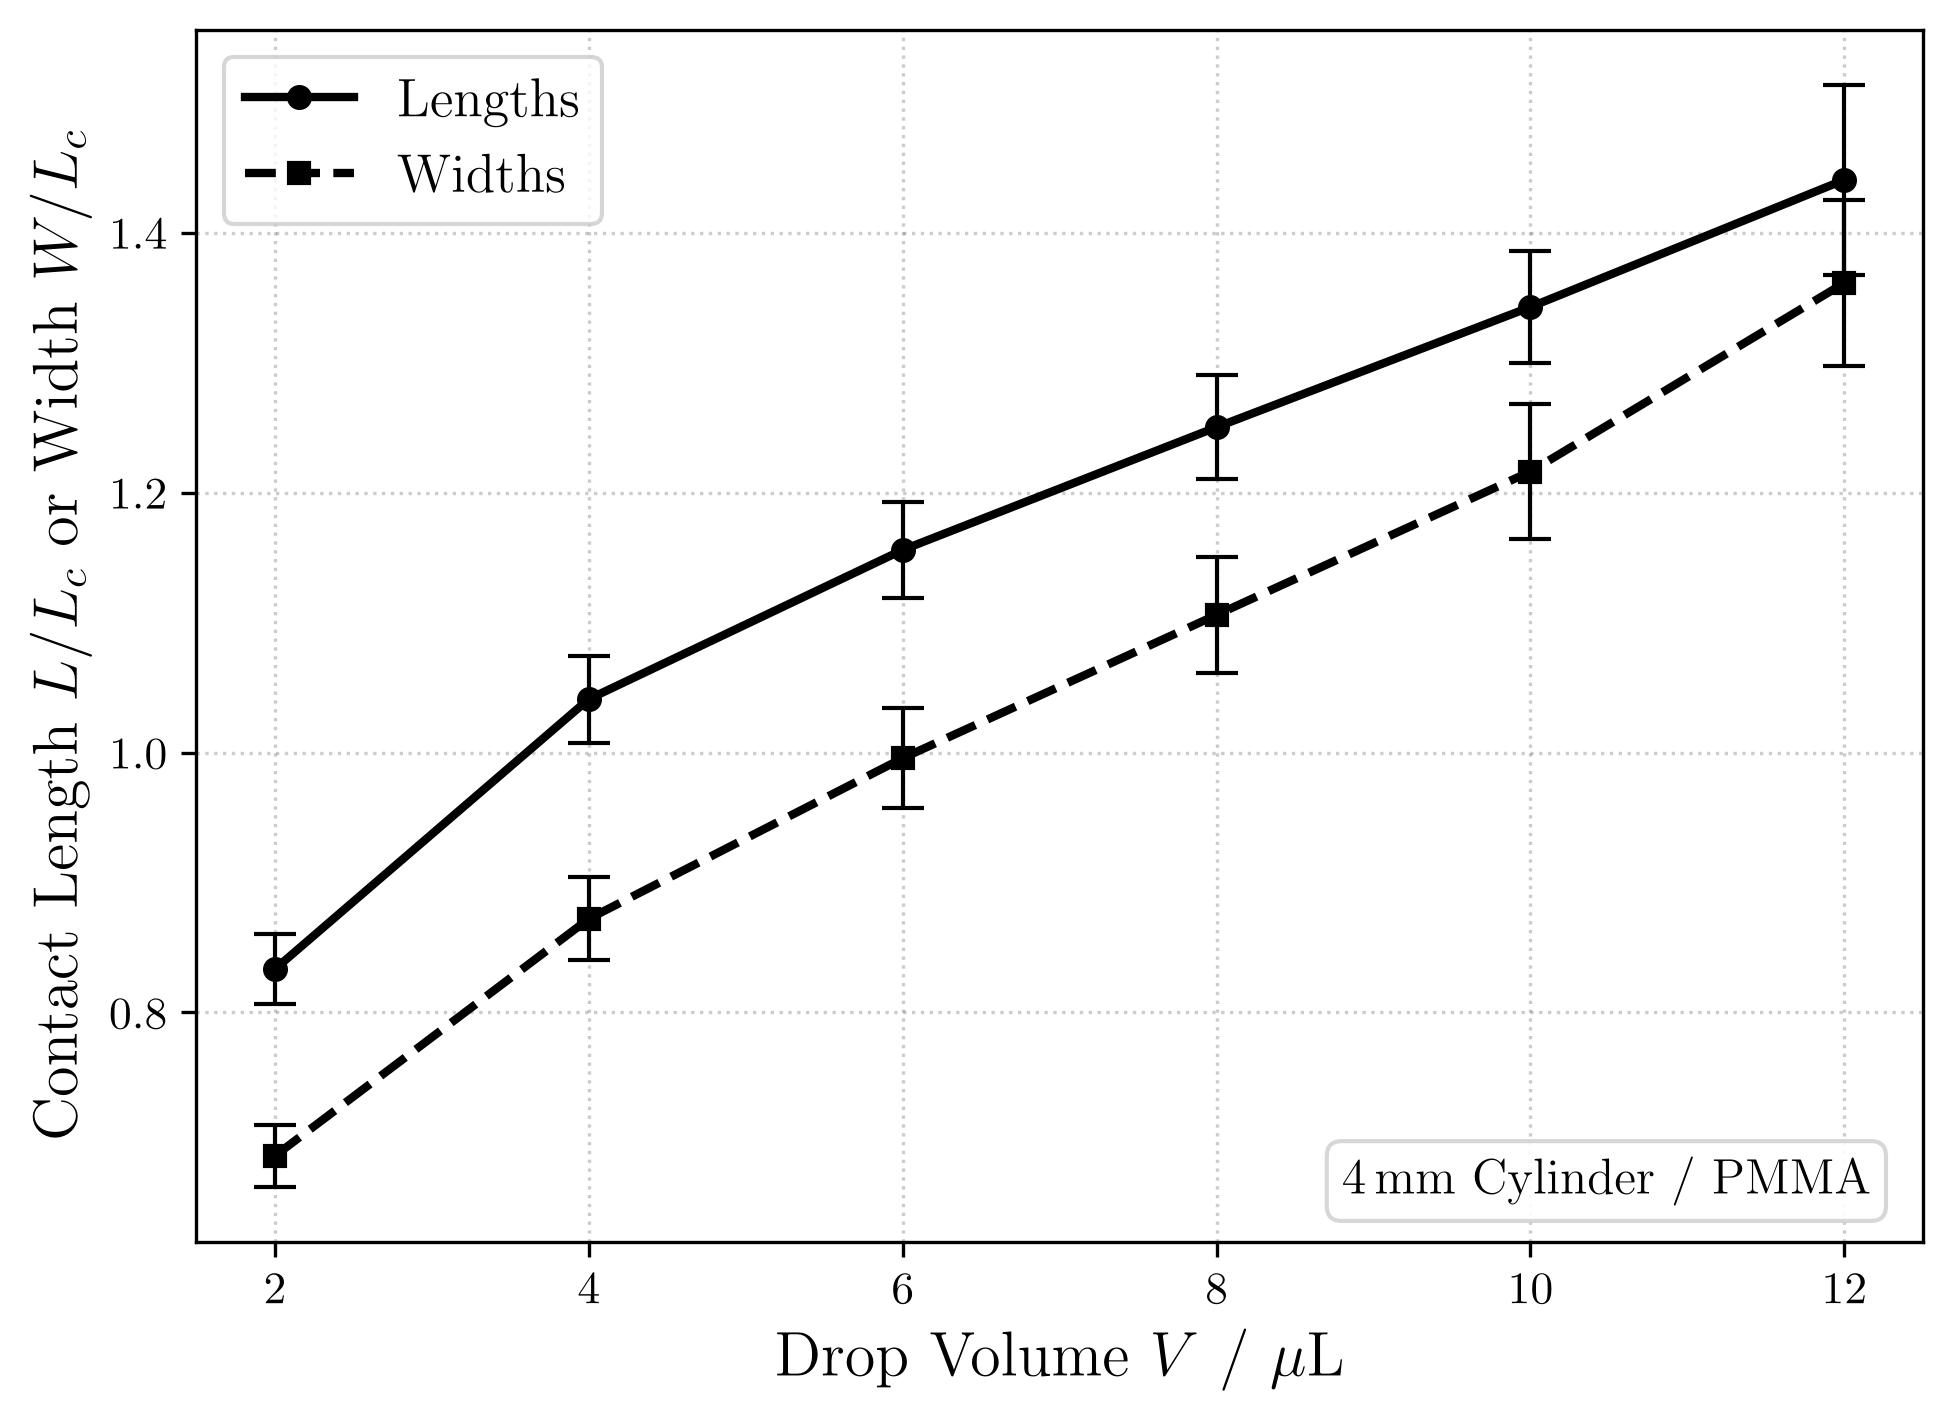
\includegraphics[width=\linewidth]{../Plots/w06_04mm_PMMA_L+W_avg.jpg}
        \caption{Contact lengths $L$ and widths $W$ on the \SI{4}{\milli\meter} PMMA cylinder. Each data point is averaged over 4 measurement repititions.}
        \label{fig:PMMA_04mm_L+W}
    \end{figure}
    Another interesting observation can be made from \ref{fig:PMMA_04mm_L+W}, where the \SI{4}{\milli\meter} PMMA cylinder is chosen for convenience: In most cases, the contact lengths $L$ are consistently larger than the widths $W$. In this regime, a carefully placed droplet then tends to align along the axis of the cylinder instead of sliding down the sides due to gravity. The mentioned regime is believed to be found for small droplet volumes $V$ with contact lengths $L$ at the order of the capillary length $L_c$, such that the surface tension dominates over the gravitational force.
    \begin{figure}[H]
        \centering
        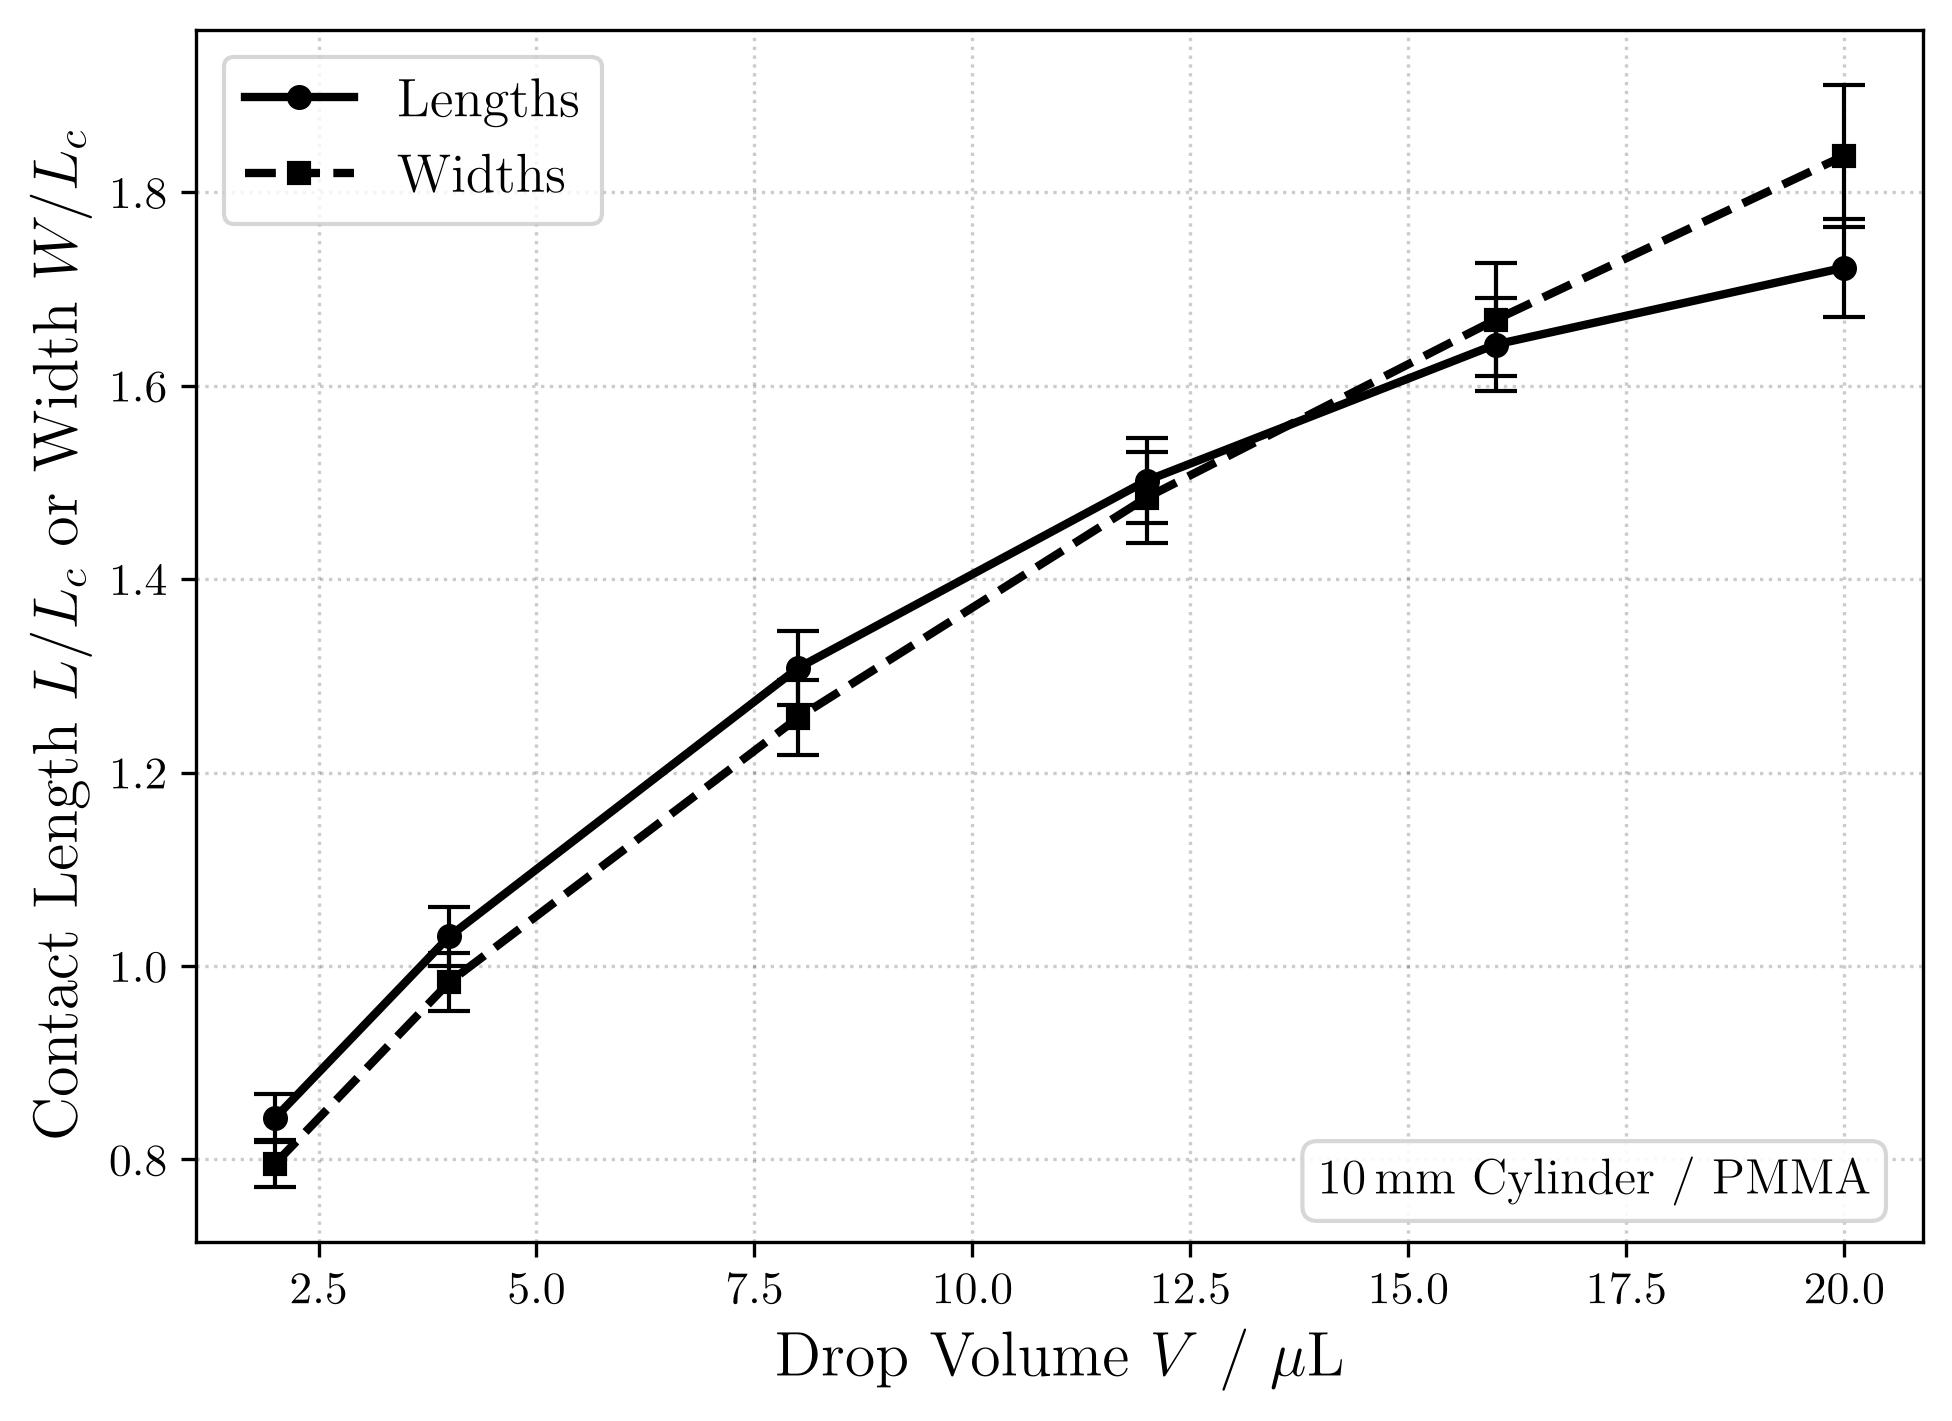
\includegraphics[width=\linewidth]{../Plots/w06_10mm_PMMA_L+W_avg.jpg}
        \caption{Contact lengths $L$ and widths $W$ on the \SI{10}{\milli\meter} PMMA cylinder. Each data point is averaged over 4 measurement repititions.}
        \label{fig:PMMA_10mm_L+W}
    \end{figure}
    The claim is furthermore supported by \cref{fig:PMMA_10mm_L+W}, which indicates that for large cylinders $D$ combined with large drop sizes $(L/L_c \gg 1)$, the gravitational force takes over and the contact width $W$ exceeds the contact length, as the droplet starts sliding down on both sides. For the \SI{10}{\milli\meter} cylinder this point $(L=W)$ is reached at a droplet volume of $V \approx\SI{13.5}{\micro\liter}$. 
    \begin{figure}[H]
        \centering
        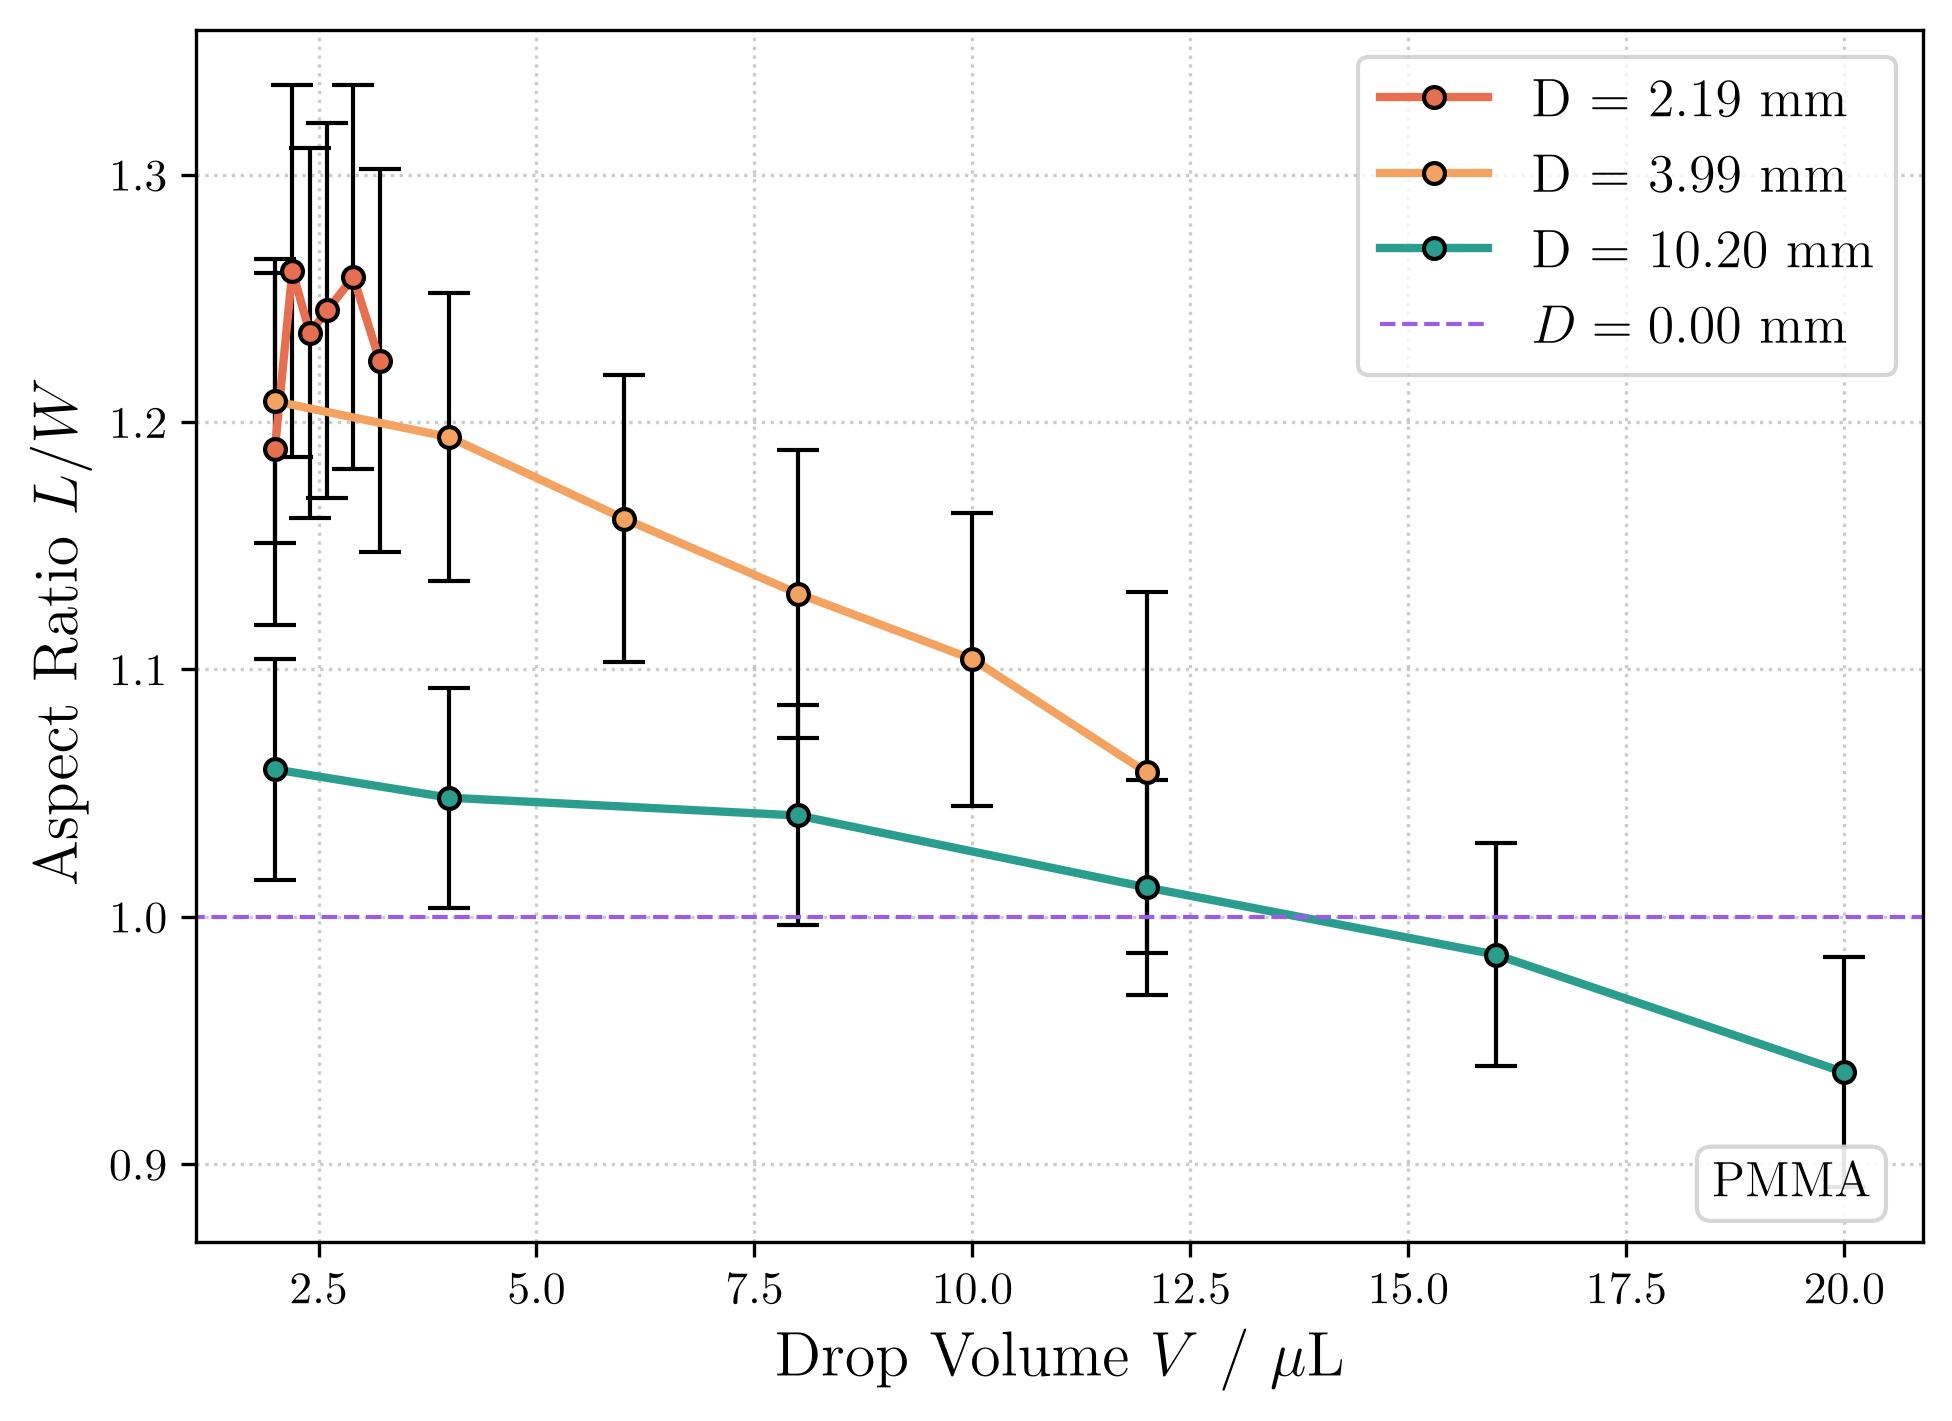
\includegraphics[width=\linewidth]{../Plots/w06_PMMA_ratios.jpg}
        \caption{Aspect ratios $L/W$ on PMMA for different diameters $D$. Each data point is averaged over 4 - 7 measurement repititions.}
        \label{fig:PMMA_ratio}
    \end{figure}
    To study the relationship of $L$ and $W$, we continue to define the aspect ratio as $L/W$, such that gravity dominates experimentally for $L/W \ll 1$ and surface tension dominates for $L/W \gg 1$ (see \cref{fig:PMMA_ratio}). \\

    Looking at \cref{fig:PMMA_ratio}, however, it is unclear if aspect ratios can be compared without accounting for the fact that a combination of higher droplet volume $V$ and cylinder diameter $D$ is just an upscaled version of the same experiment. We therefore argue that aspect ratios should not be compared against the droplet volume $V$, but the droplet volume normalized by the cylinder cross section $V / (\pi/4 \cdot D^2)$ (strictly speaking by the cylinder volume with arbitrary length). 
    \begin{figure}[H]
        \centering
        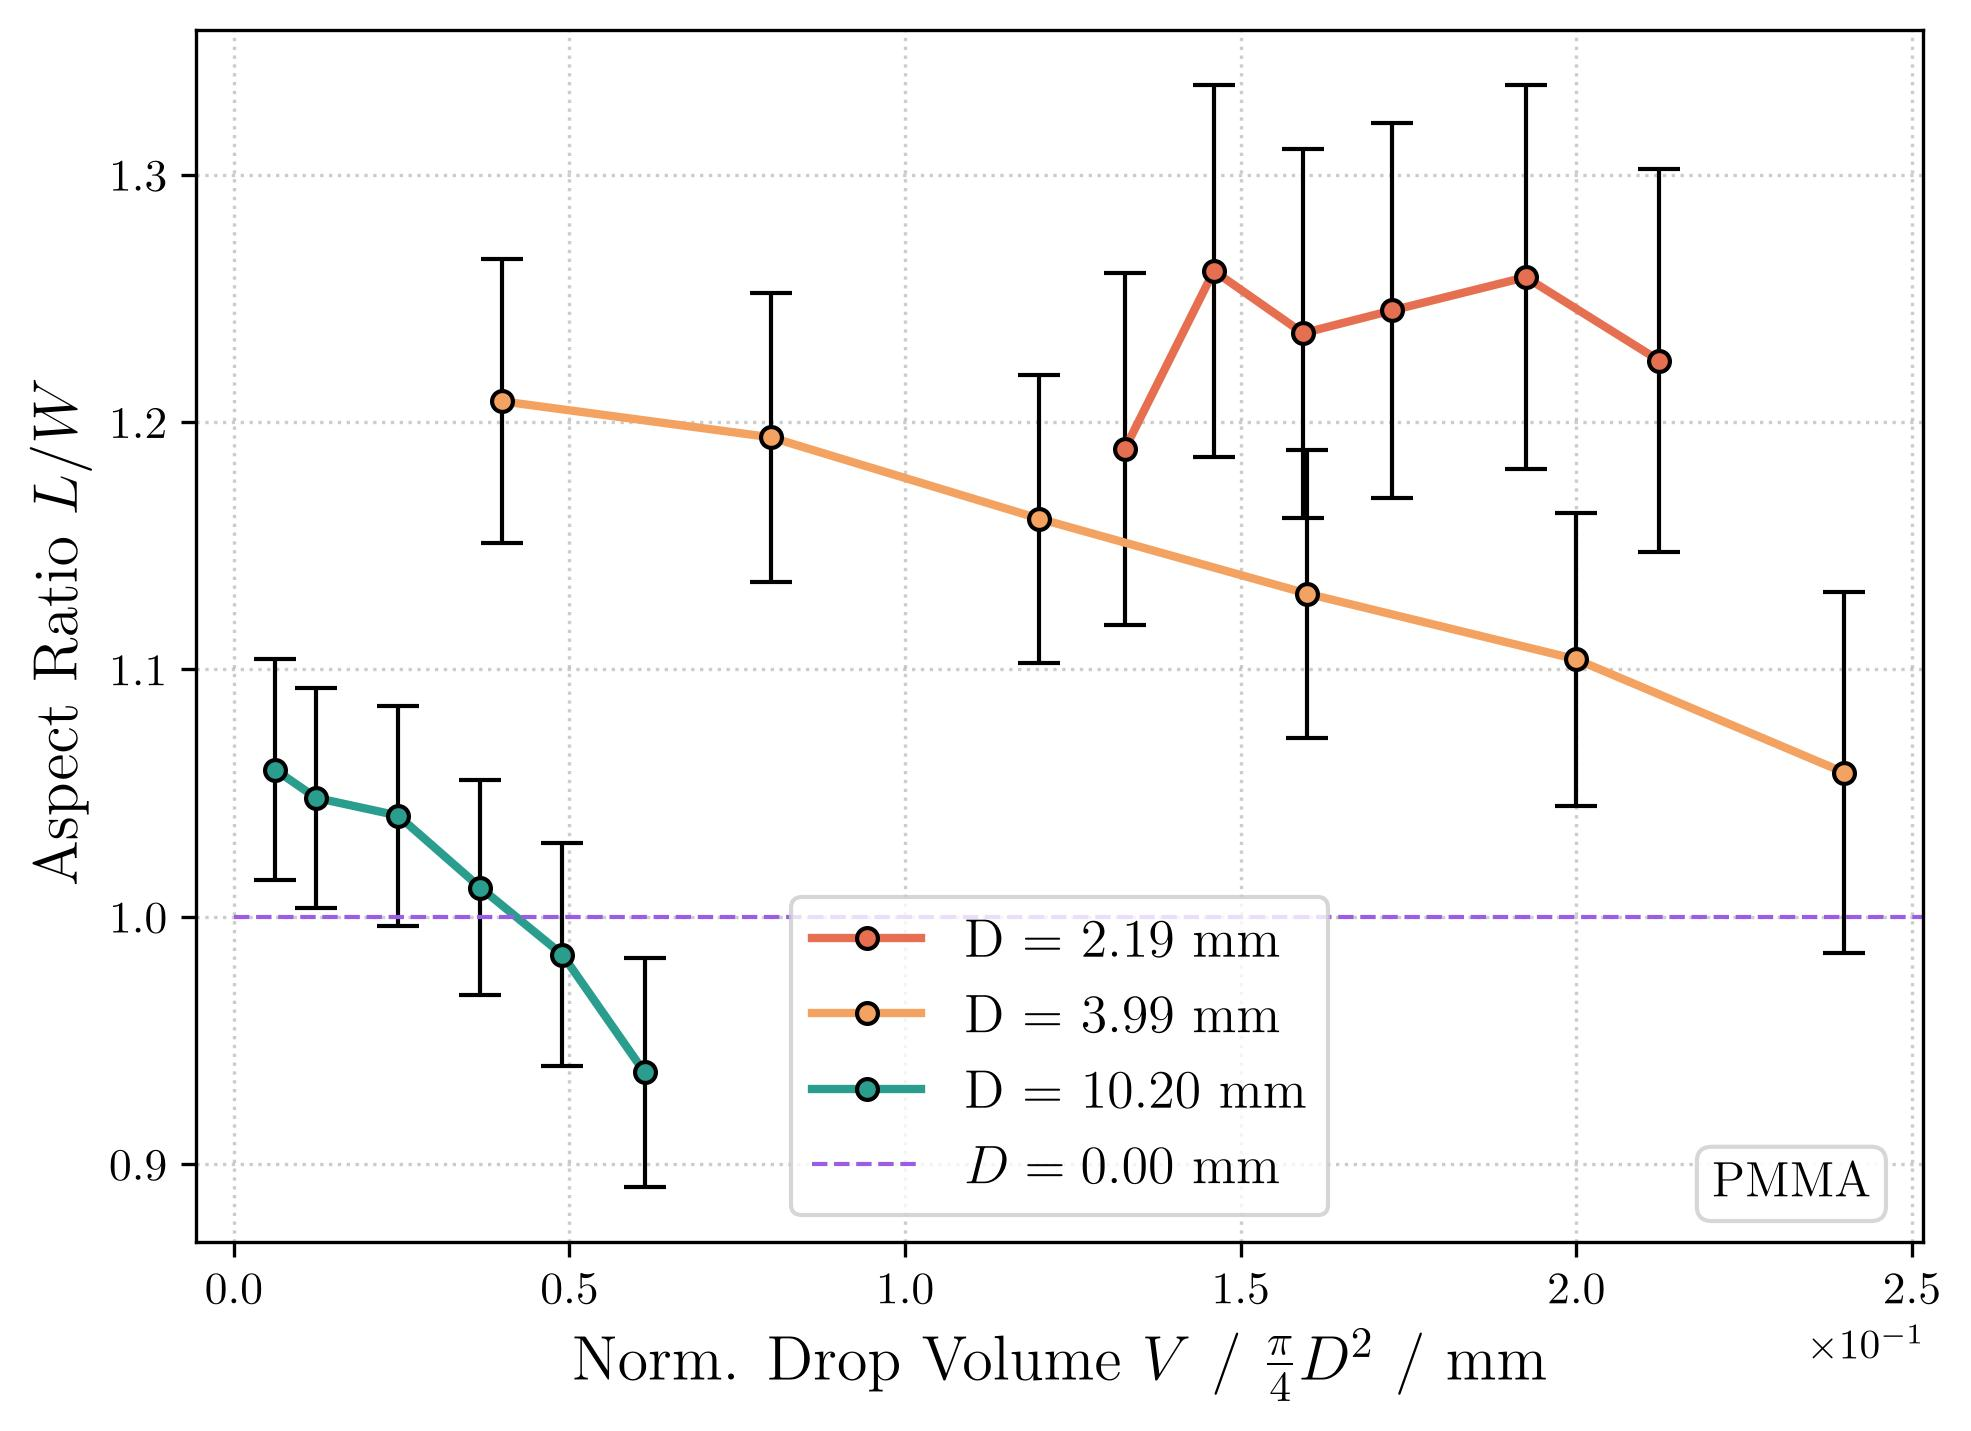
\includegraphics[width=\linewidth]{../Plots/w06_PMMA_ratios_normed.jpg}
        \caption{Aspect ratios $L/W$ on PMMA for different diameters $D$ against normed volume. Each data point is averaged over 4 - 7 measurement repititions.}
        \label{fig:PMMA_ratio_norm}
    \end{figure}
    \Cref{fig:PMMA_ratio_norm} shows the newly plotted aspect ratios and simply by the fact that the three datasets do not follow one single trajectory, we can argue that the static adhesion force is not independent of scale. This result aligns with our physical intuitions since small cylinders $\sim \SI{2}{\milli\meter}$ can hold droplets up to their own size and larger without sliding down. Large cylinders $\sim \SI{10}{\milli\meter}$, on the other hand, cannot hold droplets of half their size. This fact also becomes apparent by looking at the volume range measured for each cylinder, as each experiment was conducted until the droplets would slide off (maximum stable droplet volume). \\

    Another fact that can be inferred from both the unnormed and the normed illustration is that the aspect ratio is not a constant with respect to the droplet volume. Indeed, it heavily depends on the droplet volume chosen and it is not clear whether it can be related to physical interpretation to compare aspect ratios between cylinders for a fixed droplet volume. A comparison for fixed normed droplet volume as in \cref{fig:PMMA_ratio_norm} could be a topic for further research, once the necessary data is provided. In this case, the technical limitation to droplet volumes $V \geq \SI{2}{\micro\liter}$ does not allow for a direct comparison of normed aspect ratios. 

\subsection{Measurements on PET}

    The second material of interest is PET, a plastic that is widely used for packaging consumer products such as beverages and in industry due to its high flexibility, repellency and cheap production. \\

    We expect that PET will show properties similar to PMMA, however the experimental execution showed that PET easily falls into asymmetric shapes through droplet placement-induced vibrations, which can be traced back to stronger pinning effect and a slightly more hydrophilic profile. Another oberservation during the experiment was that tiny droplets would occasionally jump by several centimeters during droplet placement which is most likely caused by static electricity. The build-up of charge could be due to the capacitor-like design of the PET samples: The PET foil is wrapped around the PMMA cylinder, where encapsulated water and friction can load the surface with an electric charge that induces systematic error into the experiment. \\

    Taking all sources of uncertainty into consideration, it is believed that the measurements on the PET samples are only suited for qualitative analysis. For quantitative assessment, future experiments need to control the sources of uncertainty, which will be discussed more thoroughly later on. \\

    \Cref{fig:PET_L} shows the measurement of contact lengths $L$ on PET, qualitatively repeating the observation on PMMA that all measurements follow a common trajectory.
    \begin{figure}[H]
        \centering
        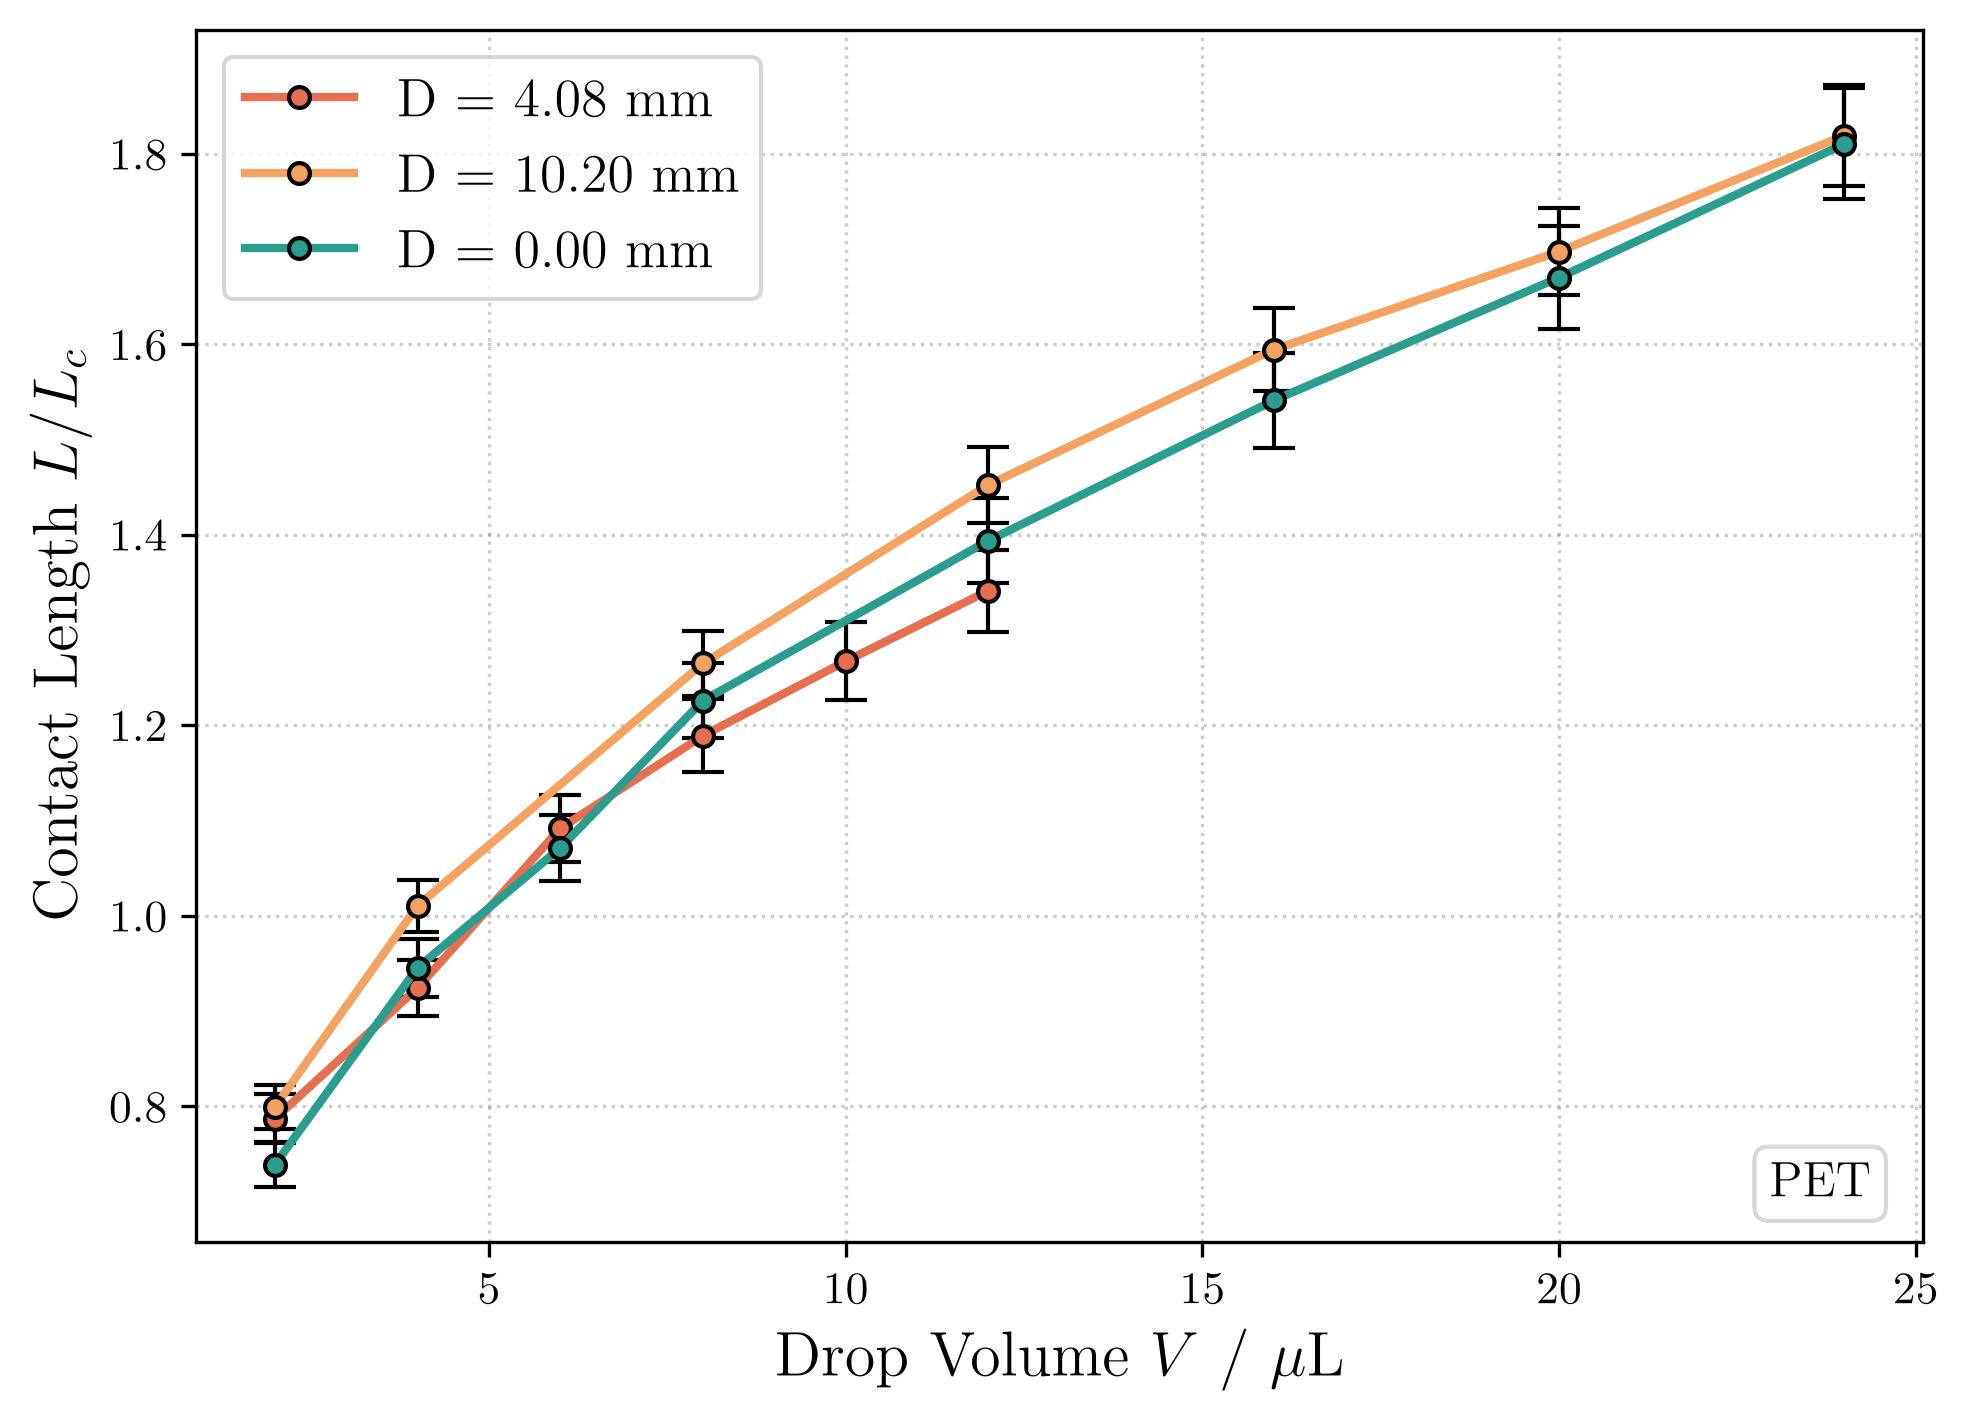
\includegraphics[width=\linewidth]{../Plots/w06_PET_L.jpg}
        \caption{Contact lengths $L$ on PET for different diameters $D$. Each data point is averaged over 4 - 7 measurement repititions.}
        \label{fig:PET_L}
    \end{figure}
    The measurements on PET contain the same anomaly that the ground measurement on the flat surface intersects with other measurements. Due to the low significance of the data, it cannot be decided whether the effect is explained by a tipping-point behaviour or a systematic error. 
    \begin{figure}[H]
        \centering
        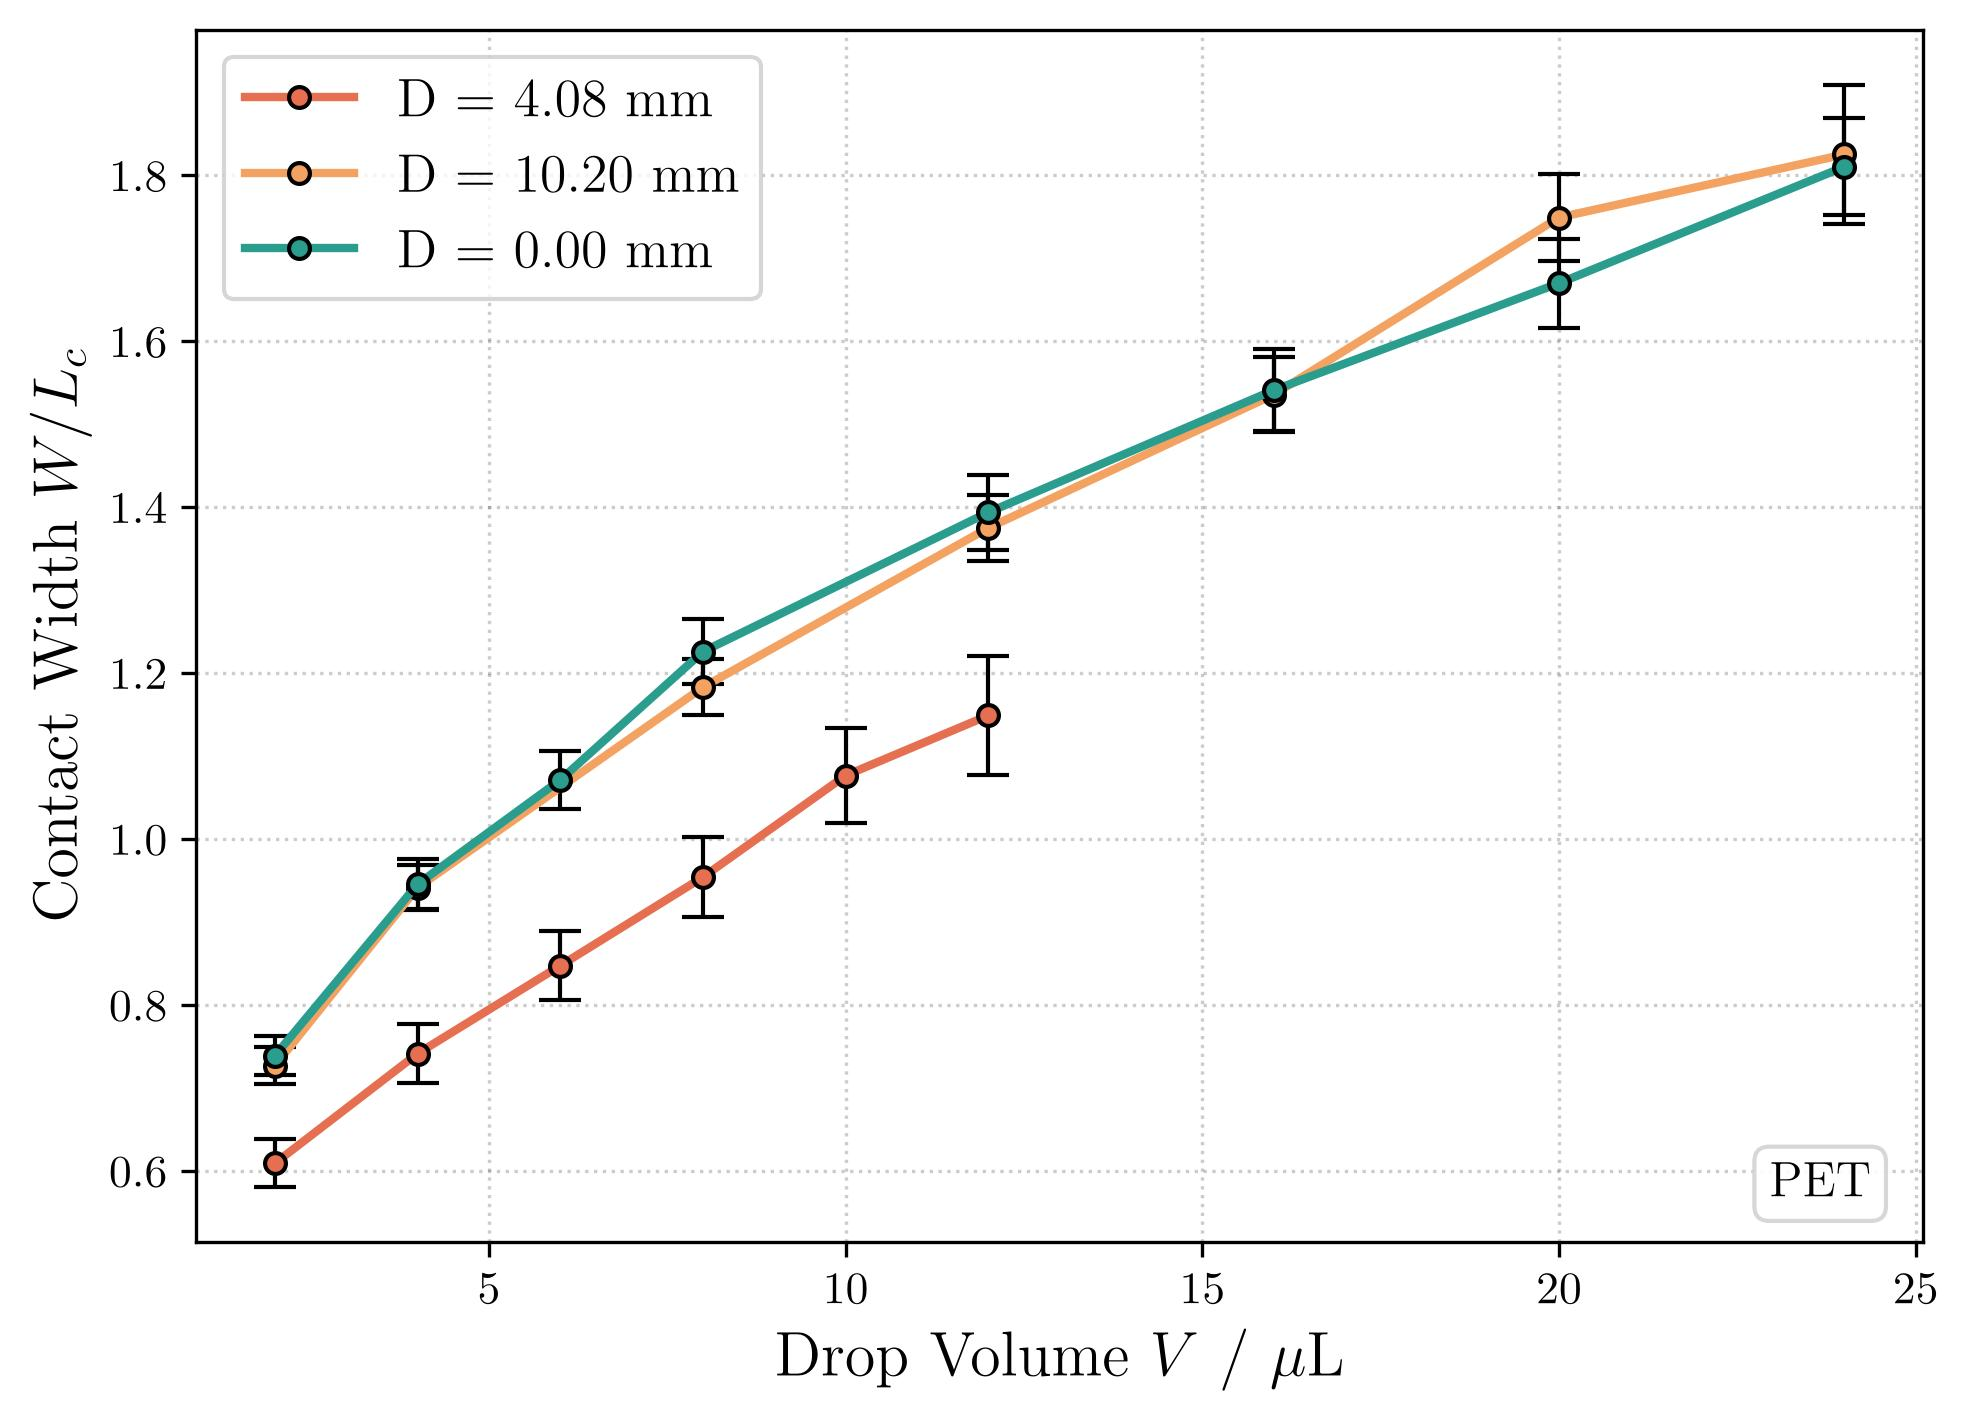
\includegraphics[width=\linewidth]{../Plots/w06_PET_W.jpg}
        \caption{Contact Widths $W$ on PET for different diameters $D$. Each data point is averaged over 4 - 7 measurement repititions.}
        \label{fig:PET_W}
    \end{figure}
    Similar to \cref{fig:PMMA_W} for PMMA, \cref{fig:PET_W} on PET shows that $W$ on the smaller cylinder follows different trajectories for each cylinder diameter, while all $L$ follow mostly the same trajectory.
    \begin{figure}[H]
        \centering
        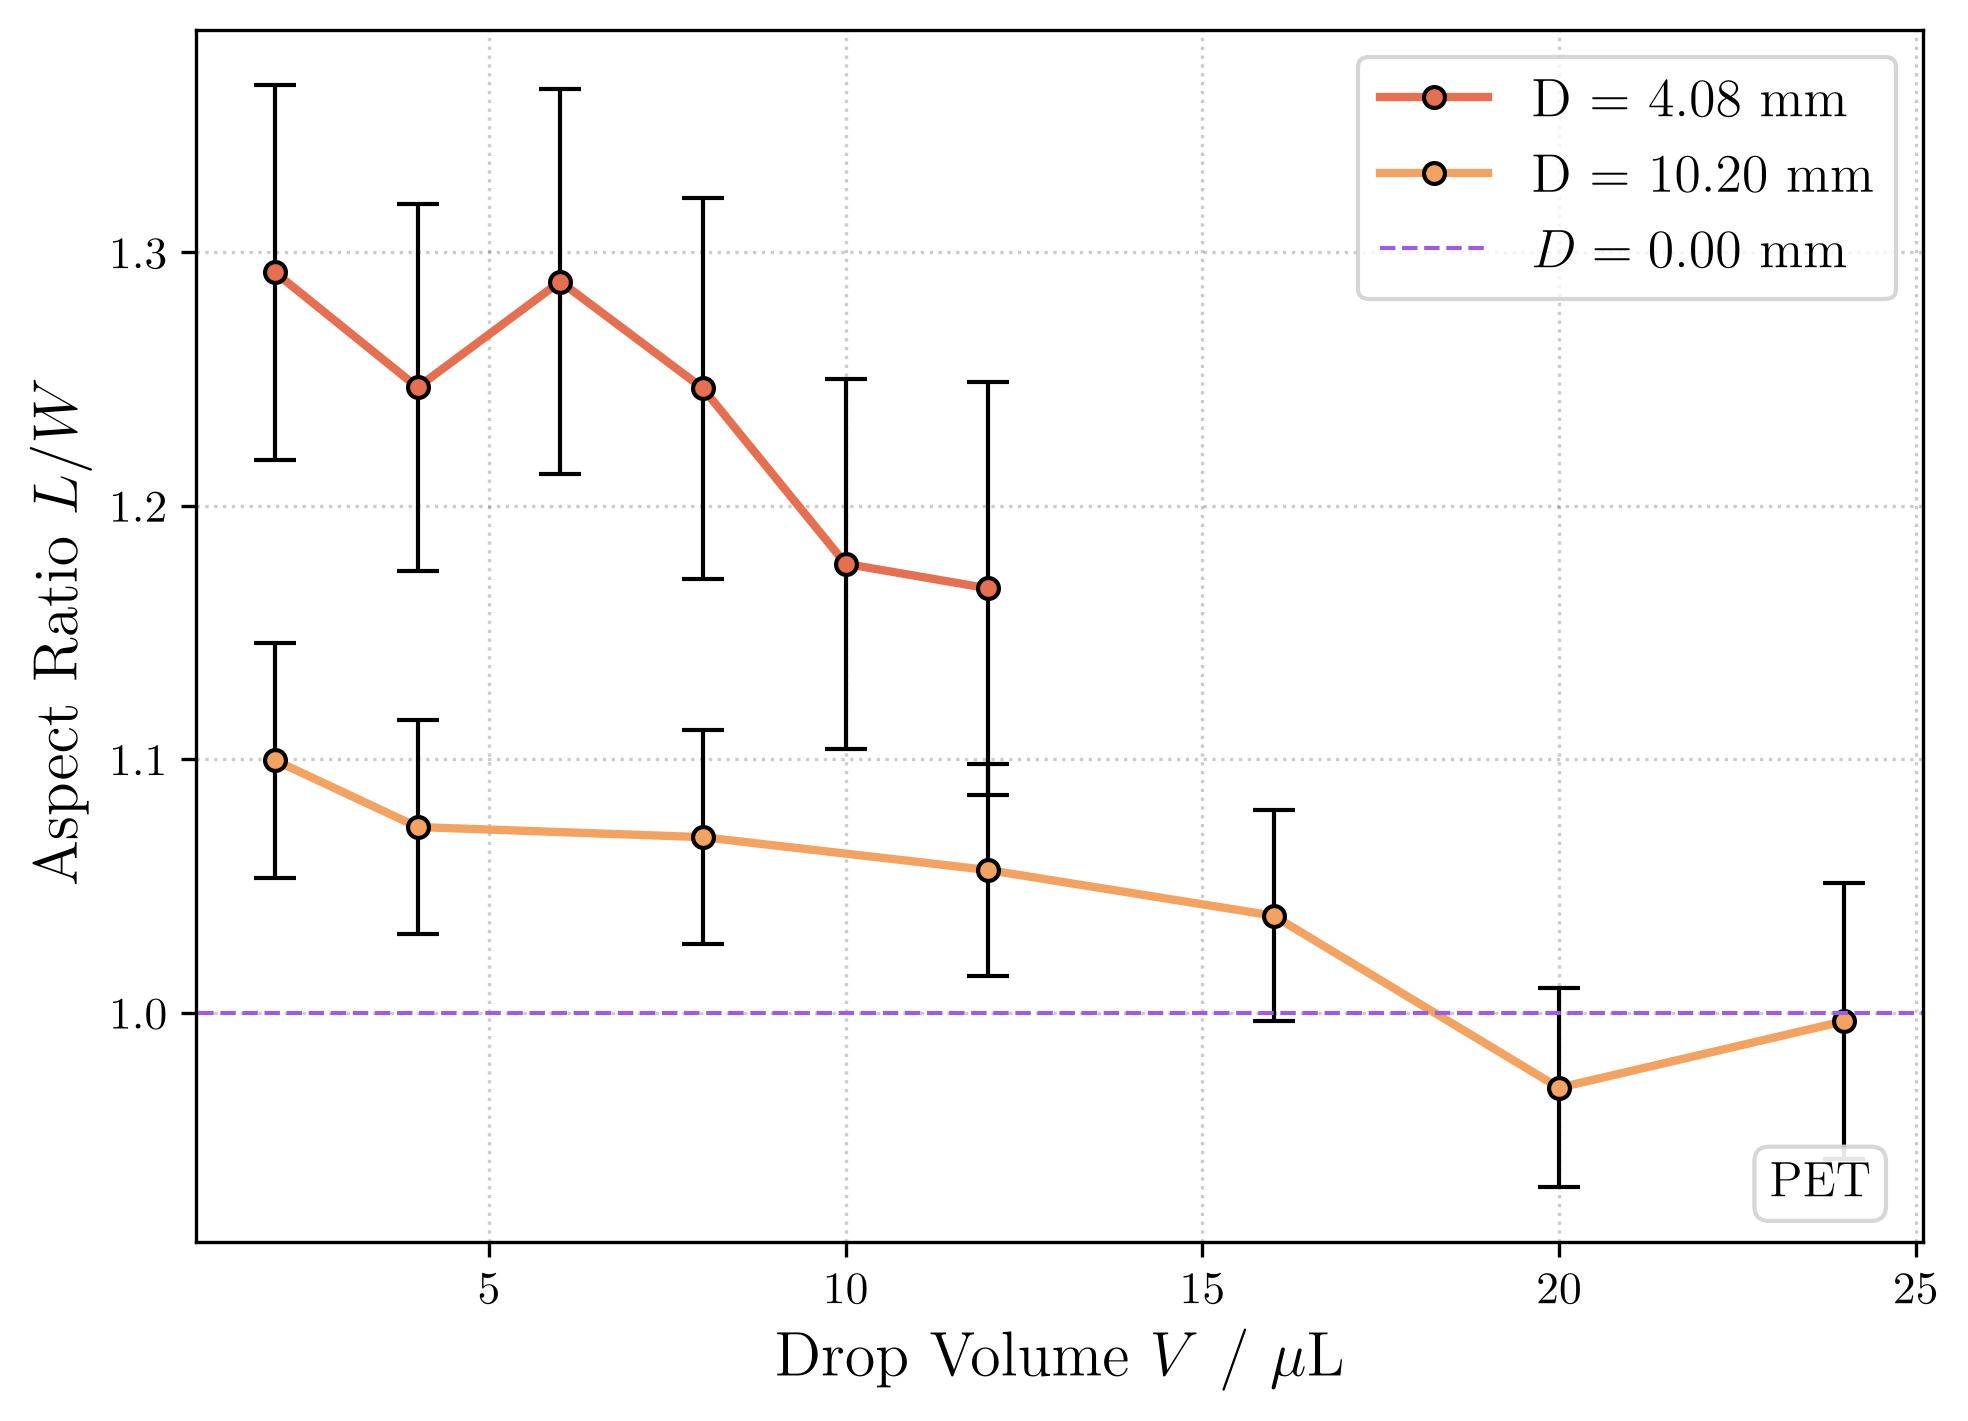
\includegraphics[width=\linewidth]{../Plots/w06_PET_ratios.jpg}
        \caption{Aspect ratios $L/W$ on PET for different diameters $D$. Each data point is averaged over 4 - 7 measurement repititions.}
        \label{fig:PET_ratio}
    \end{figure}
    The aspect ratios for the two PET cylinders are illustrated in \cref{fig:PET_ratio}. The mentioned difficulties during the measurement show up in the aspect ratio of the \SI{4}{\milli\meter} PET cylinder as the graph does not show a clear trend and suffers from high uncertainties. Since the sample quality was notably higher for the \SI{10}{\milli\meter} PET cylinder, \cref{fig:PET_ratio} depicts a much clearer downwards trend which crosses the line of $L/W = 1$ at $V \approx \SI{17}{\micro\liter}$. 
    \begin{figure}[H]
        \centering
        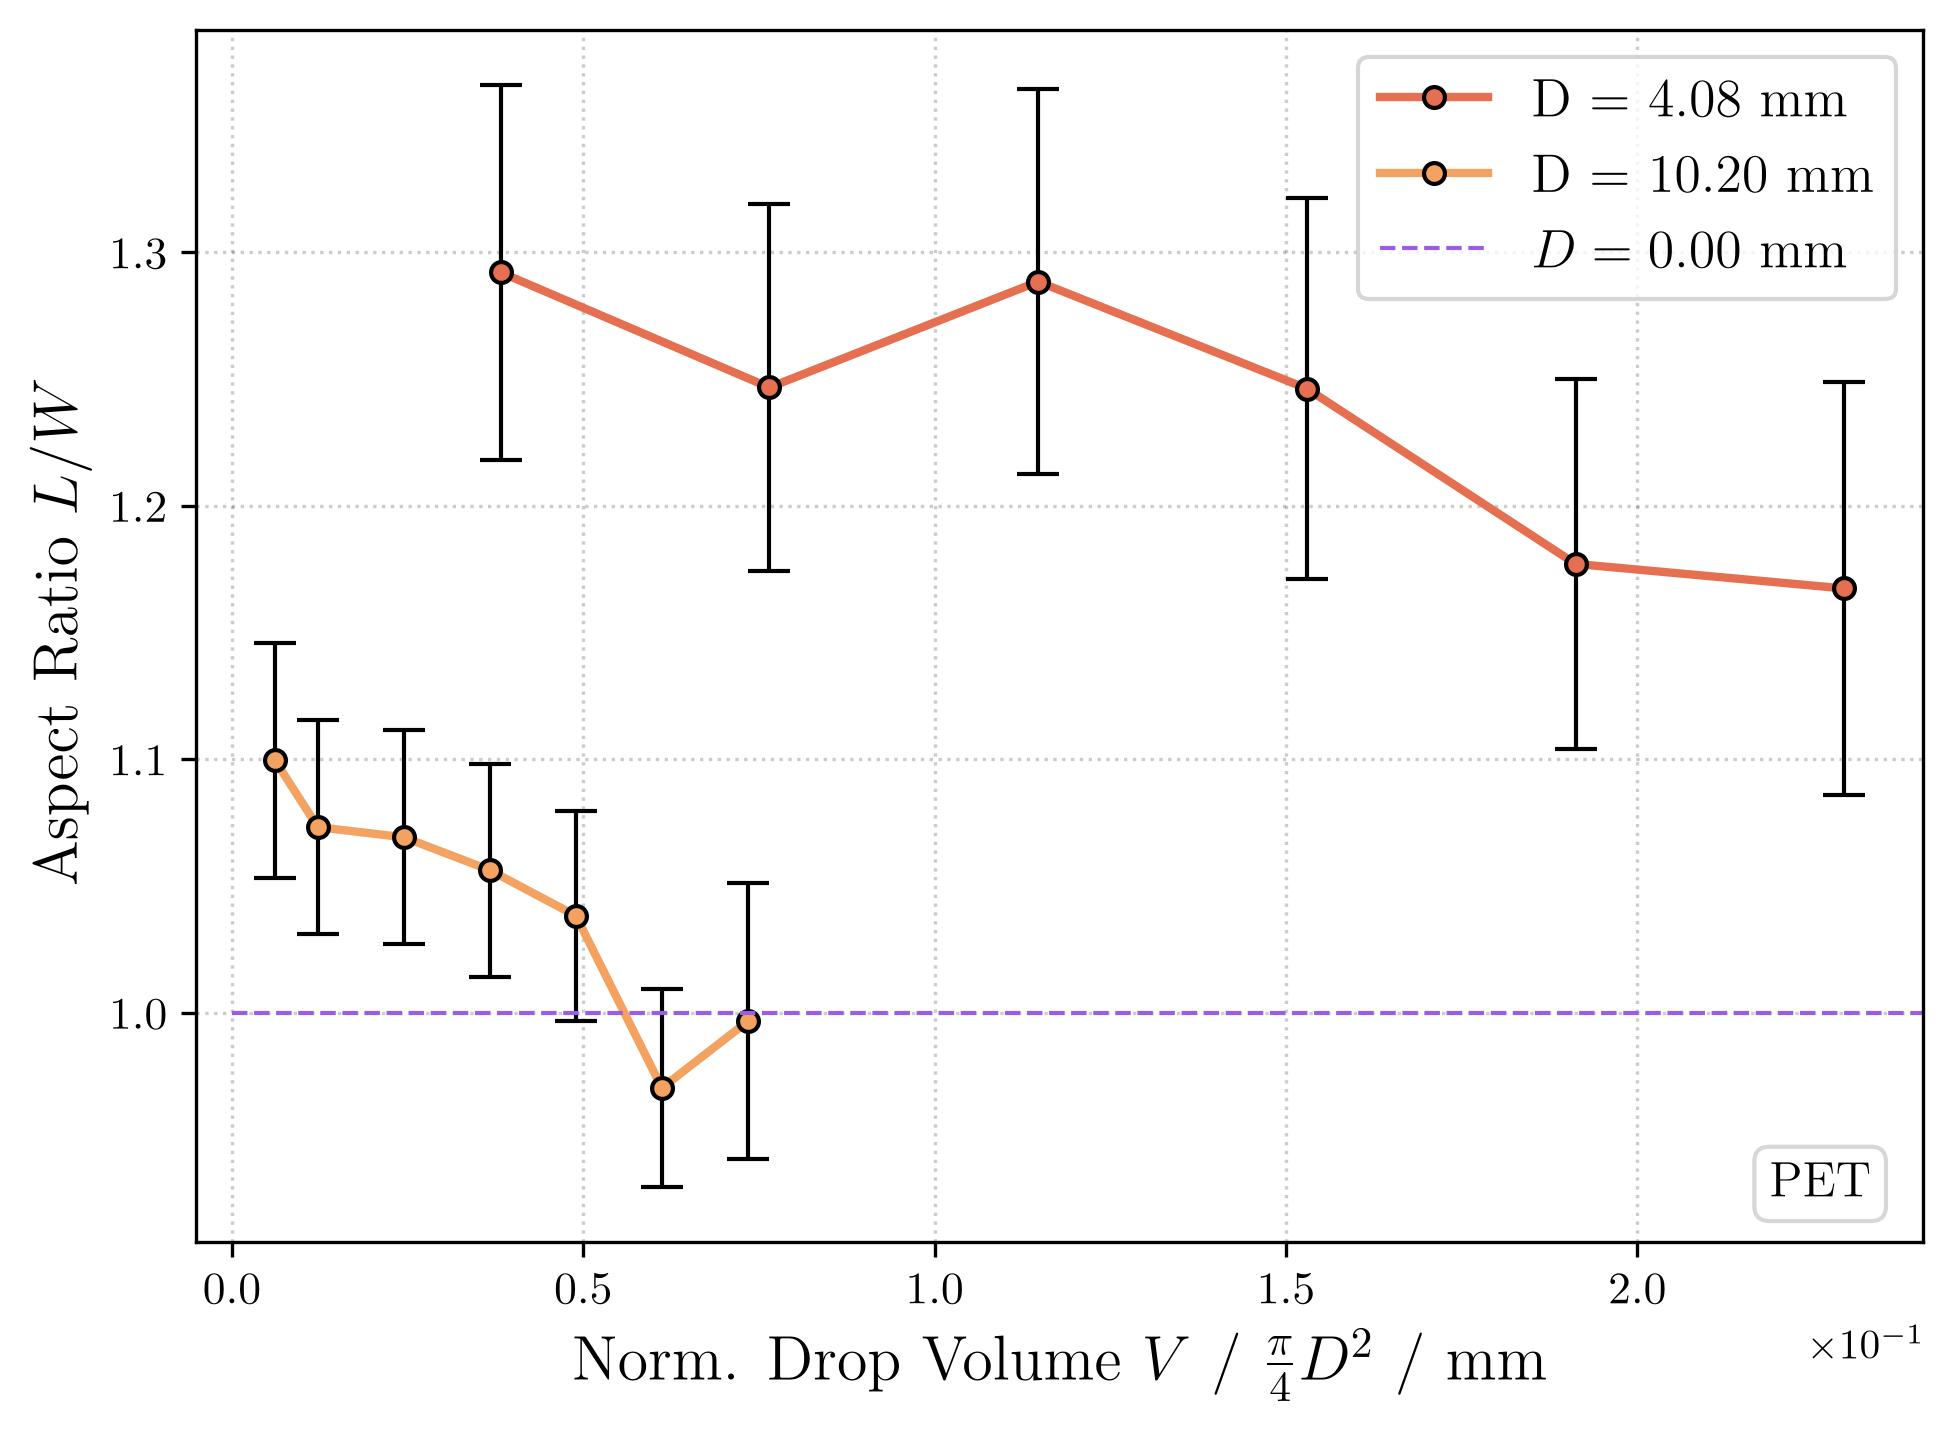
\includegraphics[width=\linewidth]{../Plots/w06_PET_ratios_normed.jpg}
        \caption{Aspect ratios $L/W$ on PET for different diameters $D$ against normed volume. Each data point is averaged over 4 - 7 measurement repititions.}
        \label{fig:PET_ratio_norm}
    \end{figure}
    The same behviour can be seen in the normed and rescaled version of the figure in \cref{fig:PET_ratio_norm}. Note that similar to the case of PMMA, the normalization of scaling still does not allow to measure the same interval of normalized volume for all cylinders, since smaller cylinders can hold much larger droplets relative to their size than larger cylinders can. Therefore, the data of the $\SI{4}{\milli\meter}$ measurement covers higher normalized volumes than the \SI{10}{\milli\meter} one as seen in the Figure. \\

    We continue to apply the linear model from \cref{eq:L_and_W_against_L0} to the contact lengths and widths (see \cref{fig:PET_04mm_fit}) and find that both cylinders and the flat PET surface obey the linear trend with proportionality constant $k \sim 1$. 
    \begin{figure}[H]
        \centering
        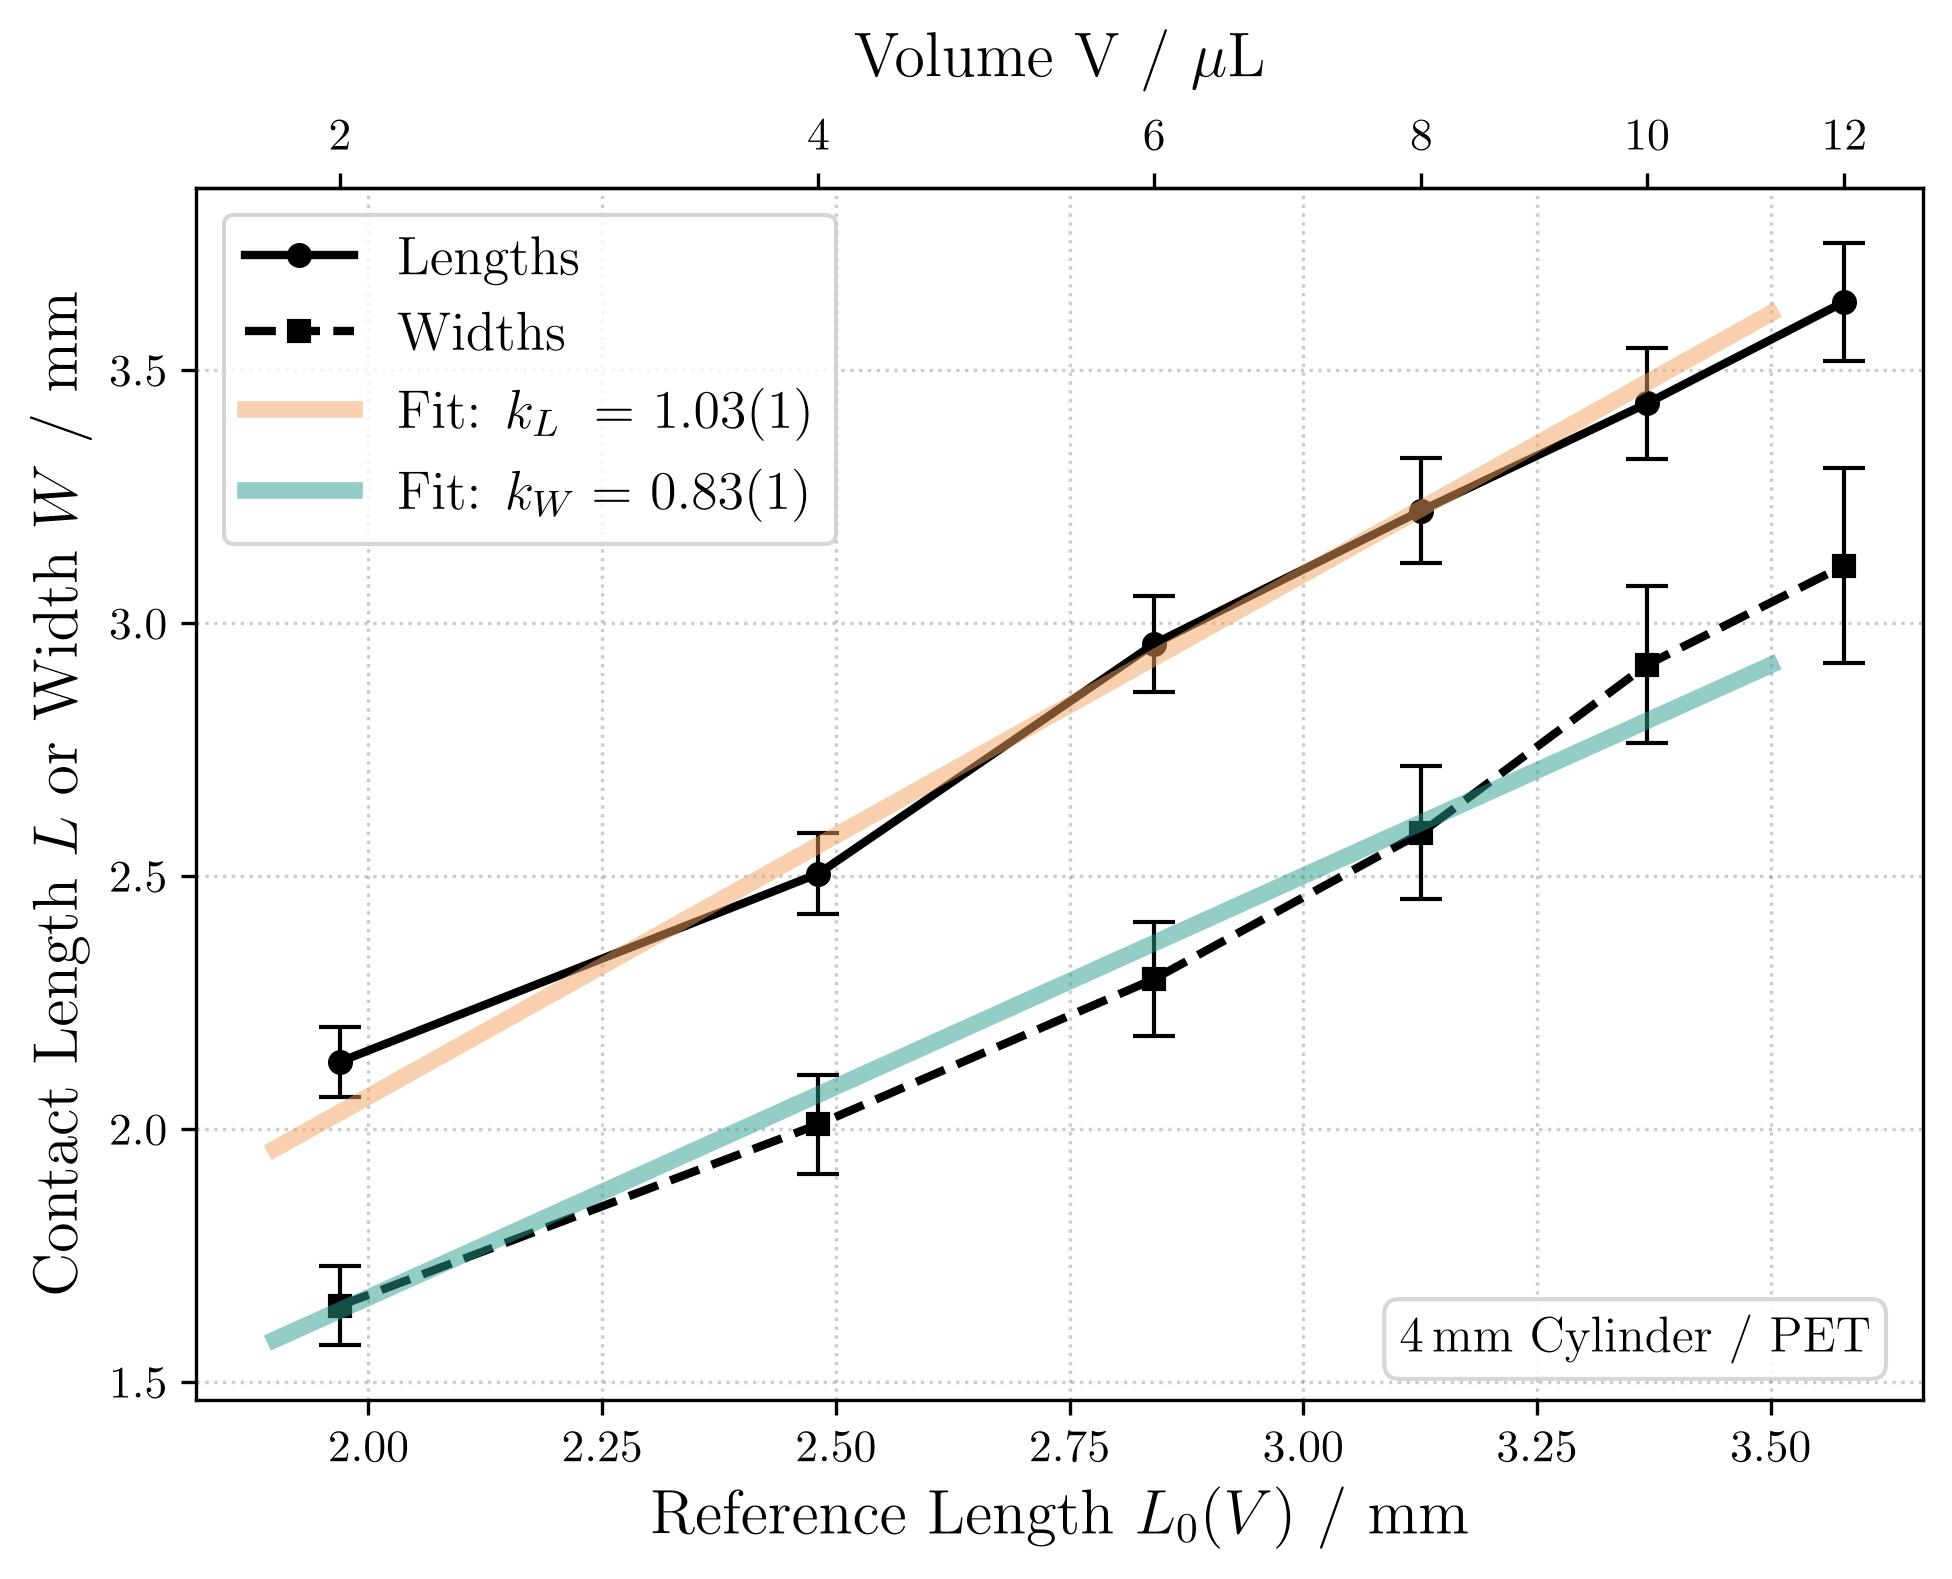
\includegraphics[width=\linewidth]{../Plots/w06_04mm_PET_L+W_fit.jpg}
        \caption{Contact lengths $L$ and widths $W$ on the \SI{4}{\milli\meter} PET cylinder, plotted against the reference length $L_0(V)$.}
        \label{fig:PET_04mm_fit}
    \end{figure}
    Looking at \cref{fig:PET_00mm_fit}, we find the best agreement between the linear model and the data for the flat PET surface as expected. In agreement with our expectation, the higher contact angles for PET materialize in the data since the slope $k_L = \num{1.060(8)}$ is smaller for PET than it was for PMMA $(k_L = \num{1.115(6)})$. The fit parameters suggest that PET exhibits more of a \enquote{rounded} shape than PMMA and therefore should have larger contact angles. 
    \begin{figure}[H]
        \centering
        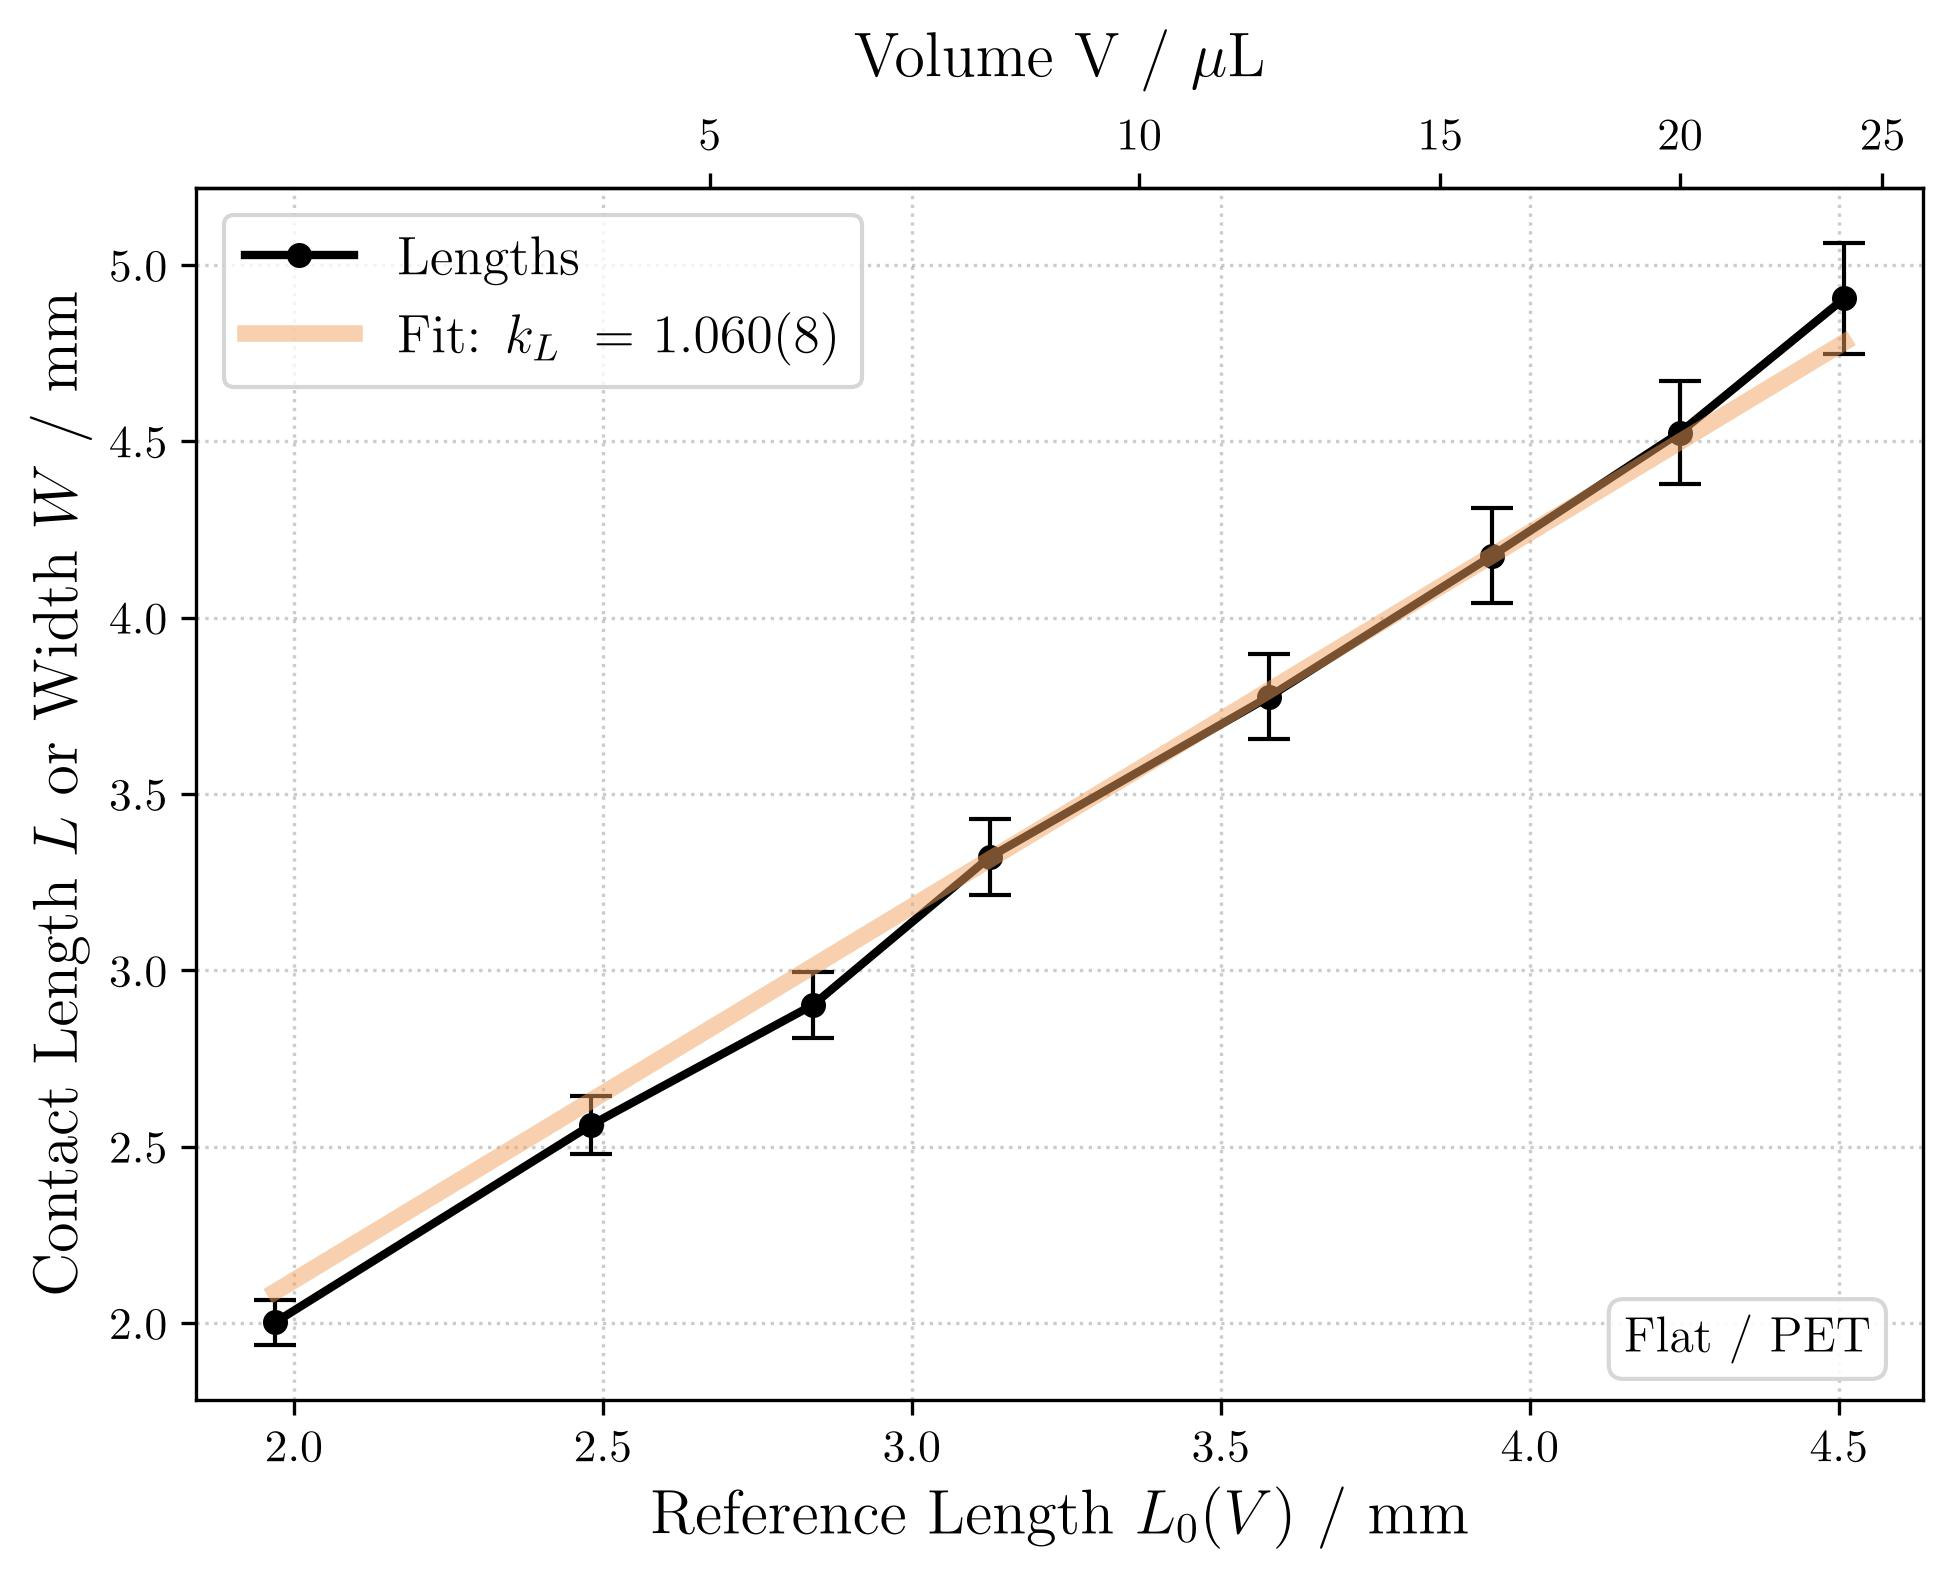
\includegraphics[width=\linewidth]{../Plots/w06_flat_PET_L_fit.jpg}
        \caption{Contact lengths $L$ on the flat PET cylinder, plotted against the reference length $L_0(V)$.}
        \label{fig:PET_00mm_fit}
    \end{figure}
    The effect can also be assessed visually by comparing two representative measurements of \SI{20}{\micro\liter} droplets for both substrates:
    \begin{figure}[H]
        \centering
        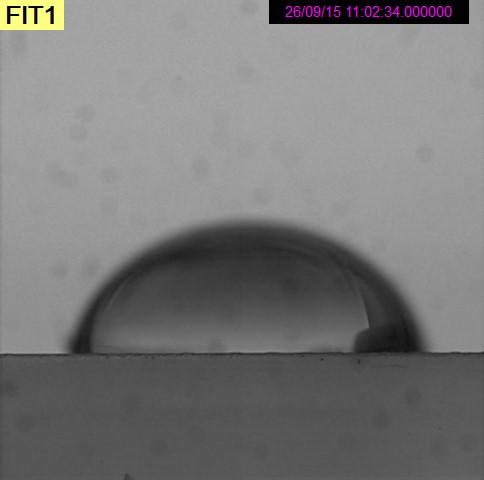
\includegraphics[width=0.48\linewidth]{../Figs/Meas_PMMA_flat_20ul.jpg}
        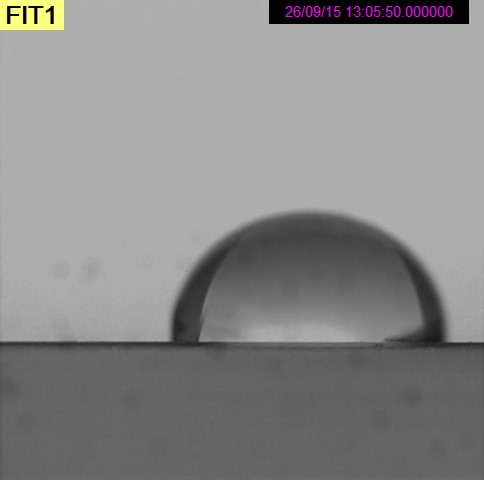
\includegraphics[width=0.48\linewidth]{../Figs/Meas_PET_flat_20ul.jpg}
        \caption{Measurements of \SI{20}{\micro\liter} droplets on PMMA (left) and PET (right). It becomes apparent that the droplet on PET is more \enquote{rounded} and possesses a larger contact angle $\theta$.}
        \label{fig:contact_angle_photo}
    \end{figure}
    The observation is furthermore supported by an a systematic error in the measurement that leads to an overestimation of PET contact lengths on the flat substrate: For this measurement, the droplet was placed at the edge of the PMMA sheet such that the droplet would interact with the surface boundary during measurement. As the droplet was attracted by the surface boundary, its shape became asymmetric and started to spread more perpendicular to the line of sight of the camera. In consequence, measured contact lengths might be exaggerated in size, an effect that has to be considered in future experiments. 

